% This is part of Mes notes de mathématique
% Copyright (c) 2011-2013,2015
%   Laurent Claessens
% See the file fdl-1.3.txt for copying conditions.


%+++++++++++++++++++++++++++++++++++++++++++++++++++++++++++++++++++++++++++++++++++++++++++++++++++++++++++++++++++++++++++
\section{Théorèmes de Sylow}
%+++++++++++++++++++++++++++++++++++++++++++++++++++++++++++++++++++++++++++++++++++++++++++++++++++++++++++++++++++++++++++

\begin{lemma}
    Soient \( H\) et \( K\) des sous-groupes finis de \( G\). Alors
    \begin{equation}
        \Card(HK)=\frac{ | H |\cdot | K | }{ | H\cap K | }.
    \end{equation}
\end{lemma} 
Attention : dans ce lemme, l'ensemble \( HK\) n'est pas spécialement un groupe. Ce serait le cas si \( H\) normaliserait \( K\), c'est à dire si nous avions \( hkh^{-1}\in K<,\forall h,k\in H\times K\).

\begin{theorem}[Théorème de Cauchy]\index{Cauchy!théorème}\index{théorème!Cauchy}       \label{ThoCauchyGpFini}
    Soit \( G\) un groupe fini et \( p\) un nombre premier divisant \( | G |\). Alors 
    \begin{enumerate}
        \item
            \( G\) contient un élément d'ordre \( p\).  
        \item
            Si \( G\) est un \( p\)-groupe, il existe un élément central d'ordre \( p\) dans \( G\).
    \end{enumerate}
\end{theorem}
Une preuve du premier point est sur \wikipedia{fr}{Théorème_de_Cauchy_(groupes)}{wikipedia}.

\begin{lemma}[Théorème de Cayley]    \label{ThoIfdlEB}   \index{Cayley!théorème}
    Si \( G\) est un groupe d'ordre \( n\) alors il est isomorphe à un sous-groupe du groupe symétrique \( S_n\).
\end{lemma}

\begin{proof}
    L'action à gauche de \( G\) sur lui-même
    \begin{equation}
        \begin{aligned}
            \varphi\colon G&\to S_n \\
            \varphi(x)g&\mapsto xg 
        \end{aligned}
    \end{equation}
    est une permutation des éléments de \( G\). Cela donne un morphisme injectif parce que si \( \varphi(x)=\varphi(y)\) nous avons \( xg=yg\) pour tout \( g\) et en particulier pour \( g=e\) nous trouvons \( x=y\).
\end{proof}

\begin{lemma}       \label{LemaQxjcm}
    Soit \( p\) un diviseur premier de \( n\). Alors le groupe symétrique \( S_n\) se plonge dans \( \GL_n(\eF_p)\).
\end{lemma}

\begin{proof}
    Soit \( \{ e_i \}\) la base canonique de \( \eF_p\). Nous avons le morphisme injectif $\varphi\colon S_n\to \GL(n,\eF)$ donné par \( \varphi(\sigma)e_i=e_{\sigma(i)}\).
\end{proof}
 
\begin{remark}  \label{RemFzxxst}
    En mettant bout à bout les lemmes \ref{ThoIfdlEB} et \ref{LemaQxjcm}, nous trouvons que si \( p\) est un diviseur premier de \( | G |\), alors \( G\) peut être vu comme un sous-groupe de \( \GL(n,\eF_p)\).
\end{remark}

\begin{definition}
    Soit \( p\) un nombre premier. Un \defe{$p$-groupe}{$p$-groupe}\index{groupe!$p$-groupe} est un groupe dont tous les éléments sont d'ordre \( p^m\) pour un certain \( m\) (dépendant de l'élément).

    Soit \( G\) un groupe fini et \( p\), un diviseur premier de $| G |$. Un \defe{\(p\)-Sylow}{$p$-Sylow}\index{Sylow!$ p$-Sylow} dans \( G\) est un \( p\)-sous-groupe d'ordre \( p^n\) où \( p^n\) est la plus grande puissance de \( p\) divisant \( | G |\).
\end{definition}
Notons que si \( p\) est un nombre premier, alors tout groupe d'ordre \( p^m\) est un \( p\)-groupe.

\begin{lemma}
    Soit \( G\) un groupe fini et \( P\), \( Q\) des \( p\)-sous-groupes. Nous supposons que \( Q\) normalise \( P\). Alors \( PQ\) est un \( p\)-sous-groupe de \( G\).
\end{lemma}

Si \( S\) est un \( p\)-Sylow, alors \( p\) ne divise pas le nombre \( | G:S |=| G |/| S |\).

\begin{proposition}     \label{Propvocmon}
    Soit le corps fini \( \eF_p=\eZ/p\eZ\) (\( p\) premier). Soit \( T\) le sous-ensemble de \( \GL_n(\eF_p)\) formé des matrices triangulaires supérieures de rang\footnote{Définition \ref{DefALUAooSPcmyK}.} \( n\) et dont les éléments diagonaux sont \( 1\). Alors \( T\) est un \( p\)-Sylow de \( \GL_n(\eF_p)\).
\end{proposition}

\begin{proof}
    Nous commençons par étudier le cardinal de \( \GL_n(\eF_p)\). Pour la première colonne, la seule contrainte à vérifier est qu'elle ne soit pas nulle. Il y a donc \( p^n-1\) possibilités. Pour la seconde, il faut ne pas être multiple de la première. Il y a donc \( p^n-p\) possibilités (parce qu'il y a \( p\) multiples possibles de la premières colonne). Pour la \( k\)-ième colonne, il faut éviter toutes les combinaisons linéaires des \( (k-1)\) premières colonnes. Il y a \( p^{k-1}\) telles combinaisons et donc \( p^n-p^{k-1}\) possibilités pour la \( k\)-ième colonne. Nous avons donc
    \begin{subequations}
        \begin{align}
            \Card\big( \GL(n,\eF_{p}) \big)&=(p^n-1)(p^n-p)\ldots(p^n-p^{n-1})\\
            &=p\cdot p^2\cdots p^{n-1}(p^n-1)(p^{n-1}-1)\ldots (p-1)\\
            &=p^{\frac{ n(n-1) }{2}}m
        \end{align}
    \end{subequations}
    où \( m\) est un entier qui ne divise pas \( p\).

    En ce qui concerne le cardinal de \( T\), le calcul est plus simple : pour la première ligne nous avons \( p^{n-1}\) choix (parce qu'il y a un \( 1\) qui est imposé sur la diagonale), pour la seconde \( p^{n-2}\), etc. En tout nous avons alors
    \begin{equation}
        | T |=p^{\frac{ n(n-1) }{2}},
    \end{equation}
    et \( T\) est un \( p\)-Sylow de \( \GL_n(\eF_p)\).
\end{proof}


\begin{proposition}
    Soit \( p\) un nombre premier. Un groupe fini \( G\) est un $p$-groupe si et seulement l'ordre de \( G\) est \( p^n\) pour un certain \( n\).
\end{proposition}

\begin{proof}
    Supposons que \( G\) est un $p$-groupe. Soit \( q\) un nombre premier divisant \( | G |\). Par le théorème de Cauchy (\ref{ThoCauchyGpFini}), le groupe \( G\) contient un élément d'ordre \( q\), soit \( g\) un tel élément. Étant donné que \( G\) est un $p$-groupe, \( g^{p^n}=g^q=e\) pour un certain \( n\). Donc $q=p^n$ et \( q=p\) parce que \( q\) est premier. Nous venons de prouver que \( p\) est le seul nombre premier qui divise \( | G |\). L'ordre de \( G\) est par conséquent une puissance de \( p\).

    Nous nous intéressons maintenant à l'implication inverse. Nous supposons que \( | G |=p^n\) pour un certain entier \( n\geq 0\). Soit \( g\in G\); nous notons \( r\) l'ordre de \( G\). Le sous-groupe \( \gr(g)\) est d'ordre \( r\), donc \( r\) divise \( | G |\) (par le théorème \ref{ThoLagrange} de Lagrange). Le nombre \( r\) est alors une puissance de \( p\).
\end{proof}

\begin{lemma}       \label{LemwDYQMg}
    Soit \( G\), un groupe fini de cardinal \( | G |=n\) et \( p\), un diviseur premier de \( n\). Nous notons \( n=p^m\cdot r\) où \( p\) ne divise pas \( r\). Soit \( H\) un sous-groupe de \( G\) et \( S\), un \( p\)-Sylow de \( G\). Alors il existe \( g\in G\) tel que 
    \begin{equation}
        gSg^{-1}\cap H
    \end{equation}
    soit un \( p\)-Sylow de \( H\).
\end{lemma}

\begin{proof}
    Nous considérons l'ensemble \( G/S\) sur lequel \( H\) agit. Si \( a\in G\), le stabilisateur de \( [a]\) dans \( G/S\) est
    \begin{subequations}
        \begin{align}
            \Stab\big( [a] \big)&=\{ h\in H\tq [ha]=[a] \}\\
            &=\{ h\in H\tq a^{-1}ha\in S\}\\
            &=aSa^{-1}\cap H.
        \end{align}
    \end{subequations}
    Nous cherchons \( a\in G\) tel que l'entier
    \begin{equation}        \label{EqZpUbWx}
        \frac{ \Card(H) }{ \Card\big( aSa^{-1}\cap H \big) }
    \end{equation}
    soit premier avec \( p\). En effet, dans ce cas le groupe \( \Stab([a])\) est un $p$-Sylow de \( H\) parce que \( | H:aSa^{-1}\cap H |\) ne divise pas \( p\). La formule des orbites (équation \eqref{EqCewSXT}) nous dit que
    \begin{equation}
        \frac{ | H | }{ | aSa^{-1}\cap H | }=\Card\big( \mO_{[a]} \big).
    \end{equation}
    Supposons que toutes les orbites aient un cardinal divisible par \( p\). Étant donné que \( G/S\) est une réunion disjointe de ses orbites, nous aurions
    \begin{equation}
        p\divides \Card(G/S)=\frac{ | G | }{ | S | }
    \end{equation}
    alors que \( S\) étant un $p$-Sylow, \( p\) ne peut pas diviser \( | G |/| S |\). Toutes les orbites n'ont donc pas un cardinal divisible par \( p\), et il existe un \( a\in G\) tel que \eqref{EqZpUbWx} soit vérifiée.
\end{proof}


\begin{theorem}[Théorème de Sylow]  \label{ThoUkPDXf}
    Soit \( G\) un groupe fini et \( p\), un diviseur premier de \( | G |\). Alors
    \begin{enumerate}
        \item
            \( G\) possède des \( p\)-Sylow.
        \item
            Tout \( p\)-sous-groupe de \( G\) est contenu dans un \( p\)-Sylow.
        \item   \label{ItemMzNRVf}
            Les \( p\)-Sylow de \( G\) sont conjugués.
        \item   \label{ItemkYbdzZ}
            Si \( n_p\) est le nombre de $p$-Sylow de \( G\), alors \( n_p\) divise \( | G |\) et \( n_p\equiv 1\mod p\).
    \end{enumerate}
\end{theorem}
\index{groupe!fini}

\begin{proof}

    % Il y a ici un début d'une preuve qui fonctionne d'une autre manière. Dans cette démonstration, N est l'ordre de G.

    %\begin{enumerate}
        %\item
         %   Nous faisons la récurrence sur l'ordre \( N\) de \( G\). Pour \( N=1\), le seul \( p\)-Sylow est le groupe entier. Si \( N>1\), nous commençons par supposer que \( G\) contient un sous-groupe propre \( H\) tel que \( \pgcd(| G:H |,p)=1\).
%
 %           Si \( G\) contient un sous-groupe propre \( H\) tel que \( \pgcd(| G:H |,p)=1\), alors \( p\) divise \( | G:H |\). En effet \( p\) divise \( N\) et \( | G:H |=| G |/| H |\). Si il n'y a pas de \( p\) dans la décomposition de \( | H |\), alors \( p\) divise encore \( | G |/| H |\). Étant donné que \( p\) est un diviseur premier de \( | H |\), le groupe \( H\) contient des \( p\)-Sylow par hypothèse de récurrence. Montrons que si \( S\) est un \( p\)-Sylow de \( H\), alors \( S\) est également un $p$-Sylow de \( G\).
%
 %           Soit \( S\), un $p$-Sylow de \( H\). Nous avons \( | S |=p^n\) où \( n\) est la plus grande puissance de \( p\) divisant \( H\). Par hypothèse, il n'y a pas de \( p\) dans la décomposition de \( | G:H |\); par conséquent \( p^n\) est également la plus grande puissance de \( p\) qui divise \( | G |\) et \( S\) est alors un $p$-Sylow de \( G\).
%
 %           Nous supposons maintenant que \( G\) ne possède pas de sous-groupe \( H\) tels que \( \pgcd(| G:H |,p)=1\).
%
 %   \end{enumerate}

    \begin{enumerate}
        \item
            
            Nous savons de la remarque \ref{RemFzxxst} que \( G\) est un sous-groupe de \( \GL_n(\eF_p)\) et que ce dernier a un $p$-Sylow par la proposition \ref{Propvocmon}. Par conséquent \( G\) possède un $p$-Sylow par le lemme \ref{LemwDYQMg}.

        \item

            Soit \( H\) un \( p\)-sous-groupe de \( G\) et \( S\), un $p$-Sylow de \( G\) (qui existe par le point précédent). Par le lemme \ref{LemwDYQMg} il existe \( a\in G\) tel que \( aSa^{-1}\cap H\) soit un $p$-Sylow de \( H\). Mais \( H\) est un \(p\)-groupe et un $p$-Sylow dans un \( p\)-groupe est automatiquement le groupe entier. Par conséquent,
            \begin{equation}
                H=aSa^{-1}\cap H
            \end{equation}
            et \( H\subset aSa^{-1}\), ce qui signifie que \( H\) est inclus à un $p$-Sylow.

        \item

            Soit \( H\) un $p$-Sylow. Nous venons de voir que si \( S\) est un $p$-Sylow quelconque, alors \( H\) est inclus au $p$-Sylow \( aSa^{-1}\) pour un certain \( a\in G\). Donc \( H\) est un $p$-Sylow inclus dans le $p$-Sylow \( aSa^{-1}\), donc \( H=aSa^{-1}\).

        \item

            Le fait que \( n_p\) divise \( n\) est parce que tous les $p$-Sylow ont le même nombre d'éléments (ils sont conjugués) et sont deux à deux disjoints. Donc ils forment une partition de \( G\) et \( | G |=n_p| S |\) si \( S\) est un $p$-Sylow quelconque.
            
            Montrons maintenant que \( n_p\) est congru à un modulo \( p\). Soit \( E\) l'ensemble des $p$-Sylow de \( G\). Le groupe \( G\) agit sur \( E\) par conjugaison. Soit \( S\) un $p$-Sylow et considérons l'ensemble
            \begin{equation}
                E_S=\{ T\in E\tq s\cdot T=T\forall s\in S \}.
            \end{equation}
            où l'action est celle par conjugaison. C'est l'ensemble des points fixes de \( E\) sous l'action de \( S\). L'ensemble \( E\) est la réunion des orbites sous \( S\) et chacune de ces orbites a un cardinal qui divise \( | S |=p^m\). Par conséquent \( | \mO_T |\) vaut \( 1\) lorsque \( T\in E_S\) et est un multiple de \( p\) sinon. Nous avons donc
            \begin{equation}
                | E |\equiv | E_S |\mod p.
            \end{equation}
            Nous voulons obtenir \( | E_S |=1\). Évidemment \( S\in E_S\) parce que si \( s\in S\) alors \( sSs^{-1}=S\). Nous voudrions montrer que \( S\) est le seul élément de \( E_S\). Soit \( T\in E_S\), c'est à dire que \( T\) est un $p$-Sylow de \( G\) tel que
            \begin{equation}
                sTs^{-1}=T
            \end{equation}
            pour tout \( s\in S\). Soit \( N\) le groupe engendré par \( S\) et \( T\). Montrons que \( T\) est normal dans \( N\). Un élément \( g\) dans \( N\) s'écrit
            \begin{equation}
                g=s_1t_1\cdots s_rt_r
            \end{equation}
            avec \( s_i\in S\) et \( t_i\in T\). Si \( t\in T\), en utilisant le fait que \( T\) est un groupe et le fait que \( S\) le normalise, nous avons
            \begin{equation}
                gtg^{-1}=s_1t_1\ldots s_rt_rtt_r^{-1}s_r^{-1}\ldots t_1^{-1}s_r^{-1}\in T.
            \end{equation}
            Donc \( T\) est un sous-groupe normal de \( N\). Mais \( S\) et \( T\) sont conjugués dans \( N\) (parce que ils sont des $p$-Sylow de \( N\)), donc il existe un élément \( a\in N\) tel que \( aTa^{-1}=S\). Mais étant donné que \( T\) est normal,
            \begin{equation}
                S=aTa^{-1}=T.
            \end{equation}
            Ceci achève la démonstration des théorèmes de Sylow.

    \end{enumerate}
\end{proof}

\begin{proposition}
    Si \( S\) est un \( p\)-Sylow dans le groupe \( G\) alors pour tout \( g\in G\), l'ensemble \( gSg^{-1}\) est encore un \( p\)-groupe.    
\end{proposition}

\begin{proof}
    Si les éléments de \( S\) sont d'ordre \( p^n\), alors nous avons
    \begin{equation}
        (gsg^{-1})^q=gs^qg^{-1}=e.
    \end{equation}
    Pour avoir \( gs^qg^{-1}=e\), il faut et suffit que \( gs^q=g\), alors \( s^q=e\), c'est à dire \( q=p^n\). Donc \( gSg^{-1}\) est encore un \( p\)-Sylow.
\end{proof}

Les deux résultats \ref{Lemcmbzum} et \ref{PropyfhTmf} proviennent de la \wikiversity{fr}{Groupe_(mathématiques)/Exercice/Premiers_résultats_sur_les_groupes_simples}{wikiversité}.
\begin{lemma}\label{Lemcmbzum}
    Soit \( G\), un groupe fini et \( p\), un nombre premier. Si \( H\) et \( K\) sont des groupes distincts d'ordre \( p\), alors \( H\cap K=\{ e \}\).
\end{lemma}

\begin{proof}
    L'ensemble \( H\cap K\) est un sous-groupe de \( H\). Par conséquent son ordre divise celui de \( H\) qui est un nombre premier. Par conséquent soit \( | H\cap K |=1\), soit \( | H\cap K |=| H |\). Dans le second cas nous aurions \( H=K\), alors que nous avons supposé que \( H\) et \( K\) étaient distincts.
\end{proof}

\begin{proposition} \label{PropyfhTmf}
    Soit \( G\) un groupe fini et \( n\) le nombre de sous-groupes d'ordre \( p\) dans \( G\). Alors le nombre d'éléments d'ordre \( p\) dans \( G\) vaut \( n(p-1)\).
\end{proposition}

\begin{proof}
    Si \( g\) est un élément d'ordre \( p\) dans \( G\), le groupe \( H\) engendré par \( g\) est d'ordre \( p\). Réciproquement si \( H\) est un groupe d'ordre \( p\), tous les éléments de \( H\setminus\{ e \}\) sont d'ordre \( p\) (parce que l'ordre d'un élément divise l'ordre du groupe). Donc l'ensemble des éléments d'ordre \( p\) dans \( G\) est la réunion des ensembles \( H\setminus\{ e \}\) où \( H\) parcours les sous-groupes d'ordre \( p\) dans \( G\). Chacun de ces ensembles possède \( p-1\) éléments et le lemme \ref{Lemcmbzum} nous assure qu'ils sont disjoints. Par conséquent nous avons \( n(p-1)\) éléments d'ordre \( p\) dans \( G\).
\end{proof}

\begin{corollary}
    Un groupe d'ordre premier est cyclique.
\end{corollary}

\begin{proof}
    Soit \( p\) l'ordre de \( G\). Le nombre de sous-groupes d'ordre \( p\) est \( n=1\) (et c'est \( G\) lui-même). La proposition \ref{PropyfhTmf} nous dit alors que le nombre d'éléments d'ordre \( p\) dans \( G\) est \( p-1\). Donc tout élément est générateur.
\end{proof}

\begin{lemma}
    Le groupe \( A_6\) n'accepte pas de sous-groupes normaux d'ordre \( 60\).
\end{lemma}

\begin{proof}
    Soit \( G\) normal dans \( A_6\), et \( a\), un élément d'ordre \( 5\) dans \( G\) (qui existe parce que \( 5\) divise \( 60\)). Soit aussi un élément \( b\) d'ordre \( 5\) dans \( A_6\). Les groupes \( \gr(a)\) et \( \gr(b)\) sont deux \( 5\)-Sylow dans \( A_6\). En effet, \( 5\) un nombre premier et est la plus grande puissance de \( 5\) dans la décomposition de \( 60\); donc \( \gr(a)\) est un \( 5\)-Sylow dans \( G\). D'autre part, l'ordre de \( A_6\) (qui est \( \frac{ 1 }{2}6!\)) ne possède également que \( 5\) à la puissance \( 1\) dans sa décomposition.

    En vertu du théorème de Sylow \ref{ThoUkPDXf}\ref{ItemMzNRVf}, les \( 5\)-Sylow \( \gr(a)\) et \( \gr(b)\) sont conjugués et il existe \( \tau\in A_6\) tel que \( b=\tau a\tau^{-1}\). Mais \( G\) étant normal dans \( A_6\), l'élément \( \tau a\tau^{-1}\) est encore dans \( G\), de telle sorte que \( b\in G\). Du coup \( G\) doit contenir tous les éléments d'ordre \( 5\) de \( A_6\).

    Les éléments d'ordre $5$ de \( A_6\) doivent fixer un des points de \( \{ 1,2,3,4,5,6 \}\) puis permuter les autres de façon à n'avoir qu'un seul cycle. Un cycle correspond à écrire les nombres \( 1,2,3,4,5\) dans un certain ordre. Ce faisant, le premier n'a pas d'importance parce qu'on considère la permutation cyclique, par exemple \( (3,5,2,1,4)\) est la même chose que \( (5,2,1,4,3)\). Le nombre de cycles sur \( \{ 1,2,3,4,5 \}\) est donc de \( 4!\), et par conséquent le nombre d'éléments d'ordre \( 5\) dans \( A_6\) est \( 6\cdot 4!=144\).

    Le groupe \( G\) doit contenir au moins \( 144\) éléments alors que par hypothèse il en contient \( 60\); contradiction.
    
\end{proof}

\begin{proposition}[\cite{Exo7Sylow}]
    Tout groupe simple d'ordre \( 60\) est isomorphe au groupe alterné \( A_5\).
\end{proposition}
Une autre preuve de ce résultat peut être trouvée sur la \wikiversity{fr}{Groupe_(mathématiques)/Exercice/Premiers_résultats_sur_les_groupes_simples}{wikiversité}. 

\begin{proof}
    Nous avons la décomposition en nombres premiers \( 60=2^2\cdot 3\cdot 5\). Déterminons pour commencer le nombre \( n_5\) de \( 5\)-Sylow dans \( G\). Le théorème de Sylow \ref{ThoUkPDXf}\ref{ItemkYbdzZ} nous renseigne que \( n_5\) doit diviser \( 60\) et doit être égal à \( 1\mod 5\). Les deux seules possibilités sont \( n_5=1\) et \( n_5=6\). Étant donné que tous les \( p\)-Sylow sont conjugués, si \( n_5=1\) alors le \( 5\)-Sylow serait un sous-groupe invariant à l'intérieur de $G$, ce qui est impossible vu que \( G\) est simple. Donc \( n_5=6\).

    Par le point \ref{ItemMzNRVf} du théorème de Sylow, le groupe \( G\) agit transitivement sur l'ensemble des \( 5\)-Sylow par l'action adjointe :
    \begin{equation}
        g\cdot S=gSg^{-1}.
    \end{equation}
    Cela donne donc un morphisme \( \theta\colon G\to S_6\). Le noyau de \( \theta\) est un sous-groupe normal. En effet si \( k\in \ker\theta\) et si \( g\in G\) nous avons
    \begin{subequations}
        \begin{align}
            (gkg^{-1})\cdot S&=gkg^{-1} Ggk^{-1}g^{-1}\\
            &=gkTk^{-1}g^{-1}\\
            &=gTg^{-1}\\
            &=S
        \end{align}
    \end{subequations}
    où \( T\) est le Sylow \( T=g^{-1}Sg\). Étant donné que \( k\in \ker\theta\) nous avons utilisé \( kTk^{-1}=aT\). Au final \( gkg^{-1}\cdot S=S\), ce qui prouve que \( gkg^{-1} \in\ker\theta\).

    Étant donné que \( \ker\theta\) est normal dans \( G\), soit est soit réduit à \( \{ e \}\) soit il vaut \( G\). La seconde possibilité est exclue parce qu'elle reviendrait à dire que \( G\) agit trivialement, ce qui n'est pas correct étant donné qu'il agit transitivement. Nous en déduisons que \( \ker\theta=\{ e \}\), que \( \theta\) est injective et que \( G\) est isomorphe à un sous-groupe de \( S_6\).

    Par ailleurs le groupe dérivé de \( G\) est un sous-groupe normal (et non réduit à l'identité parce que \( G\) est non commutatif). Donc \( D(G)=G\). Étant donné que \( G\subset S_6\), nous avons
    \begin{equation}
        G=D(G)\subset D(S_6)=A_6
    \end{equation}
    parce que le groupe dérivé du groupe symétrique est le groupe alterné (lemme \ref{LemiApyfp}).

    L'ensemble \( \theta^{-1}(A_6)\) est distingué dans \( G\). En effet si \( \sigma\in A_6\) et si \( g\in G\) nous avons
    \begin{equation}
        \theta\big( g\theta^{-1}(\sigma)g^{-1} \big)=\theta(g)\sigma \theta(g)^{-1}\in A_6.
    \end{equation}
    Nous en déduisons que \( \theta^{-1}(A_6)\) est soit \( G\) entier soit réduit à \( \{ e \}\). Si \( \theta^{-1}(A_6)=\{ e \}\), alors pour tout \( g\in G\) nous aurions \( g^2=e\) parce que \( \theta(g^2)\in A_6\). L'ordre de \( G\) étant \( 60\), il n'est pas possible que tous ses éléments soient d'ordre \( 2\). Nous en déduisons que \( \theta(G)\subset A_6\).

    Nous nommons \( H=\theta(G)\) et nous considérons l'ensemble \( X=A_6/H\) où les classes sont prises à gauche, c'est à dire 
    \begin{equation}
        [\sigma]=\{ h\sigma\tq h\in H \}.
    \end{equation}
    Évidemment \( A_6\) agit sur \( X\) de façon naturelle. Au niveau de la cardinalité,
    \begin{equation}
        \Card(X)=\frac{ | A_6 | }{ | G | }=\frac{ 360 }{ 60 }=6.
    \end{equation}
    Le groupe \( A_6\) agit sur \( X\) qui a \( 6\) éléments. Nous avons donc une application \( \varphi\colon A_6\to A_6\). Encore une fois, la simplicité de \( A_6\) montre que \( \varphi(A_6)=A_6\).

    Nous étudions maintenant \( \varphi(H)\) agissant sur \( X\). Un élément \( x\in A_6\) fixe la classe de l'unité \( [e]\) si et seulement si \( x\in H\) et par conséquent \( \varphi(H)\) est la fixateur de \( [e]\) dans \( X\). À la renumérotation près, nous pouvons identifier \( \varphi(H)\) au sous-groupe de \( A_6\) agissant sur \( \{ 1,\ldots, 6 \}\) et fixant \( 6\). Nous avons alors \( \varphi(H)=S_5\cap A_6=A_5\). Nous venons de prouver que \( \varphi\) fournit un isomorphisme entre \( A_5\) et \( H\). Étant donné que \( H\) était isomorphe à \( G\), nous concluons que \( G\) est isomorphe à \( A_6\).
\end{proof}

%+++++++++++++++++++++++++++++++++++++++++++++++++++++++++++++++++++++++++++++++++++++++++++++++++++++++++++++++++++++++++++
\section{Un peu de classification}
%+++++++++++++++++++++++++++++++++++++++++++++++++++++++++++++++++++++++++++++++++++++++++++++++++++++++++++++++++++++++++++

\begin{definition}
    Un \defe{nombre premier}{nombre!premier} est un naturel acceptant exactement deux diviseurs distincts.
\end{definition}
Avec cette définition, \( 0\) n'est pas premier, \( 1\) n'est pas premier et \( 2\) est premier.

%---------------------------------------------------------------------------------------------------------------------------
\subsection{Automorphismes du groupe \texorpdfstring{$ \eZ/n\eZ$}{Z/nZ}}
%---------------------------------------------------------------------------------------------------------------------------

Notons que \( \eZ/n\eZ=\eZ/n\eZ=\eF_n\) est un groupe pour l'addition tandis que \( (\eZ/n\eZ)^*\) est un groupe pour la multiplication. Il ne peut donc pas y avoir d'équivoque.

\begin{theorem}[\href{https://fr.wikiversity.org/wiki/Groupe\_\%28math\%C3\%A9matiques\%29/Automorphismes\_d'un\_groupe\_cyclique}{Wikiversité}%
    ]   \label{ThoozyeSn}
    Pour chaque \( x\in (\eZ/n\eZ)^*\) nous considérons l'application
    \begin{equation}
        \begin{aligned}
            \sigma_x\colon \eZ/n\eZ&\to \eZ/n\eZ \\
            y&\mapsto xy. 
        \end{aligned}
    \end{equation}
    L'application
    \begin{equation}
        \sigma\colon \big( (\eZ/n\eZ)^*,\cdot\big)\to \Aut\big( \eZ/n\eZ,+ \big)
    \end{equation}
    ainsi définie est un isomorphisme de groupes.
\end{theorem}
L'énoncé de ce théorème s'écrit souvent rapidement par 
\begin{equation}
    \Aut(\eZ/n\eZ)=(\eZ/n\eZ)^*,
\end{equation}
mais il faut bien garder à l'esprit qu'à gauche on considère le groupe additif et à droite celui multiplicatif.

\begin{proof}
    Nous notons \( [x]\) la classe de \( x\) dans \( \eZ/n\eZ\). Nous avons \( \eZ/n\eZ=[1]\). Soit \( f\) un automorphisme de \( (\eZ/n\eZ,+)\); pour tout \( r\in \eZ\) nous avons
    \begin{equation}
        f([r])=f(r[1])=rf([1])=[r]f([1]).
    \end{equation}
En particulier, vu que \( f\) est surjective, il existe un \( r\) tel que \( f([r])=[1]\). Pour un tel \( r\) nous avons \( [1]=[r]f([1])\), c'est à dire que nous avons montré que \( f([1])\) est inversible dans \(  \big( (\eZ/n\eZ)^*,\cdot\big)\). Nous montrons à présent que\footnote{Le \( \sigma\) donné ici est l'inverse de celui donné dans l'énoncé. Cela ne change évidemment rien à la validité de l'énoncé et de la preuve.}
    \begin{equation}
        \begin{aligned}
            \sigma\colon \Aut( (\eZ/n\eZ,+))&\to \big( (\eZ/n\eZ)^*,\cdot \big)<++>\\
            f&\mapsto f([1]) 
        \end{aligned}
    \end{equation}
    est un isomorphisme.

    Nous commençons par la surjectivité. Soit \( [a]\in (\eZ/n\eZ)^*\). Les élément \( [a]\) et \( [1]\) étant tous deux des générateurs de \( (\eZ/n\eZ,+)\), il existe un automorphisme de \( \eZ/n\eZ\) qui envoie \( [1]\) sur \( [a]\) par le lemme \ref{LemZhxMit}. Cela prouve la surjectivité de \( \sigma\).

    En ce qui concerne l'injectivité, considérons \( f_1\) et \( f_2\) sont de automorphismes de \( (\eZ/n\eZ,+)\) tels que \( f_1([1])=f_2([1])\). Les automorphismes \( f_1\) et \( f_2\) prennent la même valeur sur un générateur et donc sur tout le groupe. Donc \( f_1=f_2\).

    Enfin nous prouvons que \( \sigma\) est un morphisme, c'est à dire que \( \sigma(f\circ g)=\sigma(f)\sigma(g)\). Nous avons
    \begin{subequations}
        \begin{align}
            f\big( g([1]) \big)&=f\big( g([1])[1j] \big)=g([1])f([1])=\sigma(f)\sigma(g).
        \end{align}
    \end{subequations}
\end{proof}

Ce dernier résultat s'étend aux groupes cycliques.
\begin{proposition}
    Si \( G\) est un groupe cyclique d'ordre \( n\), alors
    \begin{equation}
        \Aut(G)=(\eZ/n\eZ)^*.
    \end{equation}
\end{proposition}

\begin{corollary}       \label{CorwgmoTK}
    Si \( p\) divise \( q-1\) alors \( \Aut(\eF_q)\) possède un unique sous-groupe d'ordre \( p\).
\end{corollary}

\begin{proof}
    Si \( a\) est un générateur de \( \eF_q^*\) alors le groupe
    \begin{equation}    \label{EqAdGiil}
        \gr\left( a^{\frac{ q-1 }{ p }} \right)
    \end{equation}
    est un sous-groupe d'ordre \( p\). En ce qui concerne l'unicité, soit \( S\) un sous-groupe d'ordre \( p\). Il est donc d'indice \( (q-1)/p\) dans \( \eF_q^*\) et le lemme \ref{PropubeiGX} nous enseigne que le groupe donné en \eqref{EqAdGiil} est contenu dans \( S\). Il est donc égal à \( S\) parce qu'il a l'ordre de \( S\). Le fait que \( S\) soit normal est dû au fait que \( \eF_q^*\) est abélien.
\end{proof}

%---------------------------------------------------------------------------------------------------------------------------
\subsection{Groupes abéliens finis}
%---------------------------------------------------------------------------------------------------------------------------
 
Source : \cite{FabricegPSFinis}.

Nous rappelons que l'exposant\index{exposant} d'un groupe fini est le \( \ppcm\) des ordres de ses éléments. Dans le cas des groupes abéliens finis, l'exposant joue un rôle important du fait qu'il existe un élément dont l'ordre est l'exposant. Cela est le théorème suivant.

\begin{theorem}[Exposant dans un groupe abélien fini]
    Un groupe abélien fini contient un élément dont l'ordre est l'exposant du groupe.
\end{theorem}

\begin{proof}
    Soit \( G\) un groupe abélien fini et \( x\in G\), un élément d'ordre maximum \( m\). Nous montrons par l'absurde que l'ordre de tous les éléments de \( G\) divise \( m\). Soit donc \( y\in G\), un élément dont l'ordre ne divise pas \( m\); nous notons $q$ son ordre. Vu que \( q\) ne divise pas \( m\), le nombre \( q\) possède au moins un facteur premier plus de fois que \( m\) : soit \( p\) premier tel que la décomposition de \( q\) contienne \( p^{\beta}\) et celle de \( m\) contienne \( p^{\alpha}\) avec \( \beta>\alpha\). Autrement dit,
    \begin{subequations}
        \begin{align}
            m=p^{\alpha}m'\\
            q=p^{\beta}q'
        \end{align}
    \end{subequations}
    où \( m'\) et \( q'\) ne contiennent plus le facteur \( p\). L'élément \( x\) étant d'ordre \( m\), l'élément \( x^{p^{\alpha}}\) est d'ordre \( m'\). De la même manière, l'élément \( y^{q'}\) est d'ordre \( p^{\beta}\). Étant donné que \( p^{\beta}\) et \( m'\) sont premiers entre eux, l'élément  \( x^{p^{\alpha}}y^{q'}\) est d'ordre \( p^{\alpha}m'>m\). D'où une contradiction avec le fait que \( x\) était d'ordre maximal.

    Par conséquent l'ordre de tous les éléments de $G$ divise celui de \( x\) qui est alors le \( \ppcm\) des ordres de tous les éléments de \( G\), c'est à dire l'exposant de \( G\).
\end{proof}

\begin{proposition} \label{PropfPRVxi}
    Soit \( G\) un groupe abélien fini et \( x\in G\), un élément d'ordre maximum. Alors
    \begin{enumerate}
        \item
            Il existe un morphisme \( \varphi\colon G\to \gr(x)\) tel que \( \varphi(x)=x\).
        \item   \label{ItemKRYwjU}
            Il existe un sous-groupe \( K\) de \( G\) tel que \( G=\gr(x)\oplus K\).
    \end{enumerate}
\end{proposition}

\begin{proof}
    Nous notons \( a\) l'ordre de \( x\) qui est également l'exposant du groupe \( G\).

    Nous allons prouver la première partie par récurrence sur l'ordre du groupe. Si \( G=\gr(x)\), alors c'est évident. Soit \( H\) un sous-groupe propre de \( G\) contenant \( x\) et tel que le problème soit déjà résolu pour \( H\) : il existe un morphisme \( \varphi\colon H\to \gr(x)\) tel que \( \varphi(x)=x\). Soit \( y\in G\setminus H\), d'ordre \( b\). Nous allons trouver un morphisme $\hat\varphi\colon \gr(H,y)\to \gr(x) $ telle que \( \hat\varphi(x)=x\).

    Pour cela nous commençons par construire les applications suivantes :
    \begin{equation}
        \begin{aligned}
            \tilde \varphi\colon \eZ/b\eZ\times H&\to \gr(x) \\
            (\bar k,h)&\mapsto x^{kl}\varphi(h) 
        \end{aligned}
    \end{equation}
    où \( l\) est encore à déterminer, et
    \begin{equation}
        \begin{aligned}
            p\colon \eZ/b\eZ\times H&\to \gr(y,H) \\
            (\bar k,h)&\mapsto y^kh. 
        \end{aligned}
    \end{equation}
    Pour que \( \tilde \varphi\) soit bien définie, il faut que \( a\) divise \( bl\). L'application \( p\) est bien définie parce que \( \bar k\) est pris dans \( \eZ/b\eZ\) et que \( b\) est l'ordre de \( y\).

    Nous allons construire le morphisme \( \hat \varphi\) en considérant le diagramme 
    \begin{equation}
    \xymatrix{%
    \ker(p) \ar@{^{(}->}[r]        &   \eZ/b\eZ\times H\ar[d]_{\tilde \varphi}\ar[r]^p&\gr(y,H)\ar[ld]^{\hat \varphi}\\
          &   \gr(x)
       }
    \end{equation}
    que l'on voudra être commutatif. Vu que \( p\) est surjective, les théorèmes d'isomorphismes nous disent que
    \begin{equation}
        \gr(y,H)\simeq\frac{ \eZ/b\eZ\times H }{ \ker p }.
    \end{equation}
    Si \( [\bar k,h]\) est la classe de \( (\bar k,h)\) modulo \( \ker(p)\) alors nous voudrions définir \( \hat \varphi\) par
    \begin{equation}        \label{EqeesVxc}
        \hat\varphi\big( [\bar k,h] \big)=\tilde \varphi(\bar k,h).
    \end{equation}
    Pour que cela soit bien définit, il faut que si \( (\bar r,z)\in \ker p\),
    \begin{equation}
        \hat\varphi\big( [\bar k\bar r,hz] \big)=\hat\varphi\big( [\bar k,h] \big),
    \end{equation}
    c'est à dire que \( \tilde \varphi(\bar r,z)=e\). Du coup la définition \eqref{EqeesVxc} n'est bonne que si et seulement si
    \begin{equation}
        \ker(p)\subset\ker(\tilde\varphi ).
    \end{equation}
    Nous pouvons obtenir cela en choisissant bien \( l\).

    Déterminons d'abord le noyau de \( p\). Pour cela nous considérons un nombre \( \beta\) divisant \( b\) tel que \( \gr(y)\cap H=\gr(y^{\beta})\). Nous aurons \( p(\bar k,h)=e\) si et seulement si \( y^h=e\). En particulier \( h=y^{-k}\in\gr(y)\cap H=\gr(y^{\beta})\). Si \( h=(y^{\beta})^m=y^{m\beta}\), alors \( k=-m\beta\) et nous avons
    \begin{equation}
        \ker(p)=\{ (-m\beta,y^{m\beta})\tq m\in \eZ \}.
    \end{equation}
    En plus court : \( \ker(p)=\gr(\beta,y^{-\beta})\). Nous devons donc fixer \( l\) de telle sorte que \( \tilde \varphi(\beta,y^{-\beta})=e\). Étant donné que \( \varphi\) prend ses valeurs dans \( \gr(x)\), il existe un entier \( \alpha\) tel que \( \varphi(y^{-\beta})=x^{\alpha}\); en utilisant cet \( \alpha\), nous écrivons
    \begin{equation}
        \tilde \varphi(\beta,y^{-\beta})=x^{\beta l}\varphi(y^{-\beta})=x^{\beta l+\alpha}.
    \end{equation}
    Par conséquent nous choisissons \( l=-\alpha/\beta\). Nous devons maintenant vérifier que ce choix est légitime, c'est à dire que \( a\) divise \( bl\) et que \( \alpha/\beta\) est un entier.

    Étant donné que \( y\) est d'ordre \( b\),
    \begin{equation}
        e=\varphi(y^b)=\varphi(y^{-\beta b/\beta})=\varphi(y^{-\beta})^{b/\beta}=x^{b\beta/\alpha}.
    \end{equation}
    Par conséquent \( a\) divise \( \frac{ b\alpha }{ \beta }=-bl\).

    Pour voir que \( l\) est entier, nous nous rappelons que \( a\) est l'exposant de \( G\) (parce que \( x\) est d'ordre maximum) et que par conséquent \( b\) divise \( a\). Mais \( a\) divise \( \alpha\frac{ b }{ \beta }\). Donc \( \alpha/\beta\) est entier.

    Nous passons maintenant à la seconde partie de la preuve. Nous considérons un morphisme \( \varphi\colon G\to \gr(x)\) tel que \( \varphi(x)=x\). La première partie nous en assure l'existence. Nous montrons que 
    \begin{equation}
        \begin{aligned}
            \psi\colon G&\to \gr(x)\oplus \ker(\varphi) \\
            g&\mapsto \big( \varphi(g),g\varphi(g)^{-1} \big) 
        \end{aligned}
    \end{equation}
    est un isomorphisme. D'abord \( g\varphi(g)^{-1}\) est dans le noyau de \( \varphi\) parce que \( \varphi(g)^{-1}\) étant dans \( \gr(x)\), et \( \varphi\) étant un morphisme,
    \begin{equation}
        \varphi\big( g\varphi(g)^{-1} \big)=\varphi(g)\varphi(g)^{-1}=e.
    \end{equation}
    L'application \( \psi\) est un morphisme parce que, en utilisant le fait que \( G\) est abélien,
    \begin{subequations}
        \begin{align}
            \psi(g_1g_2)&=\big( \varphi(g_1g_2),g_1g_2\varphi(g_1g_2)^{-1} \big)\\
            &=\big( \varphi(g_1)\varphi(g_2),g_1\varphi(g_1)^{-1}g_2\varphi(g_2)^{-1} \big)\\
            &=\psi(g_1)\psi(g_2).
        \end{align}
    \end{subequations}
    L'application \( \psi\) est injective parce que si \( \psi(g)=(e,e)\) alors \( \varphi(g)=e\) et \( g\varphi(g)^{-1}=e\), ce qui implique \( g=e\).

    Enfin \( \psi\) est surjective parce qu'elle est injective et que les ensembles de départ et d'arrivée ont même cardinal. En effet par le premier théorème d'isomorphisme (théorème \ref{ThoPremierthoisomo}) appliqué à \( \varphi\) nous avons
    \begin{equation}
        | G |=| \gr(x) |\cdot | \ker(\varphi) |.
    \end{equation}
\end{proof}

\begin{theorem} \label{ThoRJWVJd}
    Tout groupe abélien fini (non trivial) se décompose en
    \begin{equation}
        G\simeq \eZ/d_1\eZ\oplus\ldots\oplus \eZ/d_r\eZ
    \end{equation}
    avec \( d_1\geq 1\) et \( d_i\) divise \( d_{i+1}\) pour tout \( i=1,\ldots, r-1\).

    De plus la liste \( (d_1,\ldots, d_r)\) vérifiant ces propriétés est unique.
\end{theorem}

\begin{proof}
    Soit \( x_1\) un élément d'ordre maximal dans \( G\). Soit \( n_1\) son ordre et
    \begin{equation}
        H_1=\gr(x_1)=\eF_{n_1}.
    \end{equation}
    D'après la proposition \ref{PropfPRVxi}\ref{ItemKRYwjU}, il existe un supplémentaire \( K_1\) tel que \( G=\eF_{n_1}\oplus K_1\). Si \( K_1=\{ 1 \}\) on s'arrête et on garde \( G=\eF_{n_1}\). Sinon on continue de la sorte en prenant \( x_2\) d'ordre maximal dans \( K_1\) etc.

    Nous devons maintenant prouver l'unicité de cette décomposition. Soit
    \begin{equation}
        G=\eF_{d_1}\oplus\ldots\oplus \eF_{d_r}=\eF_{s_1}\oplus\ldots\oplus \eF_{s_q}.
    \end{equation}
    L'exposant de \( G\) est \( d_r\) et \( s_q\). Donc \( d_r=s_q\). Les complémentaires étant égaux nous avons
    \begin{equation}
        \eF_{d_1}\oplus\ldots\oplus \eF_{d_{r-1}}=\eF_{s_1}\oplus\ldots\oplus \eF_{s_{q-1}}.
    \end{equation}
    En continuant nous trouvons \( r=q\) et \( d_i=s_i\).
\end{proof}
 
%---------------------------------------------------------------------------------------------------------------------------
\subsection{Groupes d'ordre \texorpdfstring{$ pq$}{pq}}
%---------------------------------------------------------------------------------------------------------------------------
\index{quotient!de groupes}\index{sous-groupe!normal}

Soit \( G\) un groupe d'ordre \( pq\) où \( p\) et \( q\) sont des nombres premiers distincts. Nous supposons que \( p<q\). Montrons que \( G\) ne possède qu'un seul \( q\)-Sylow. Soit \( n_q\) le nombre de \( q\)-Sylow; par les théorèmes de Sylow nous avons
\begin{equation}
    n_q=1\mod q
\end{equation}
et \( n_q\) divise \( | G |=pq\). Donc \( n_q\) vaut \( p\), \( q\) ou \( 1\). Avoir \( n_q=p\) n'est pas possible parce que \( n_q=1\mod q\) et \( p<q\). Avoir \( n_q=q\) n'est pas possible non plus, pour la même raison. Donc \( n_q=1\). Notons \( H\) cet unique \( q\)-Sylow de \( G\).

Notons que cet unique \( q\)-Sylow est un sous-groupe normal dans \( G\) qui n'est égal ni à \( \{ 1 \}\) ni à \( \{ G \}\) parce que
\begin{equation}
    1<p=| H |<pq=| G |.
\end{equation}
Par conséquent \( G\) n'est pas simple.

\begin{theorem} \label{ThoLnTMBy}
    Soit \( G\) un groupe d'ordre \( pq\) où \( q>p\) sont des nombres premiers distincts\footnote{Le cas \( p=q\) sera traité par la proposition \ref{PropssttFK}.}. 

    Si \( q\neq 1\mod p\) alors \( G\) est cyclique et plus précisément \( G\simeq \eZ/pq\eZ\).

    Si \( q=1\mod p\), alors soit \( G\) est abélien et est le groupe cyclique \( G\simeq \eZ/pq\eZ\), soit \( G\) n'est pas abélien et
    \begin{equation}    \label{EqNuuTRE}
        G\simeq \eZ/q\eZ\times_{\varphi}\eZ/p\eZ
    \end{equation}
    où \( \varphi(\bar 1)\) est d'ordre \( p\) dans \( \Aut(\eZ/q\eZ)\).

    De plus tous les produits semi-directs non triviaux de la forme \eqref{EqNuuTRE} sont isomorphes entre eux, c'est à dire que si \( \eZ/q\eZ\times_{\varphi}\eZ/p\eZ\) et \( \eZ/q\eZ\times_{\varphi'}\eZ/p\eZ\) sont d'ordre \( pq\), alors ils sont isomorphes.

    En particulier si \( p\) et \( q\) sont premiers entre eux, le produit est direct.
\end{theorem}
\index{sous-groupe!distingué}
\index{groupe!fini}
\index{anneau!\( \eZ/n\eZ\)}
\index{nombre!premier}

\begin{proof}
    Soient \( H\), un \( q\)-Sylow et \( K\), un \( p\)-Sylow de \( G\). Ils existent parce que \( p\) et \( q\) sont des diviseurs premiers de \( | G |\) (théorème de Sylow \ref{ThoUkPDXf}). Si \( n_q\) est le nombre de \( q\)-Sylow dans \( G\) alors \( n_q\) divise \( | G |\) et \( n_q=1\mod q\). Donc d'abord \( n_q\) vaut \( 1\), \( p\) ou \( q\). Ensuite \( n_q=q\) est exclu par la condition \( n_q=1\mod q\); la possibilité \( n_q=p\) est également impossible parce que \( p=1\mod q\) est impossible avec \( p<q\). Donc \( n_q=1\) et \( H\) est normal dans \( G\).

    L'ensemble \( H\cap H\) est un sous-groupe à la fois de \( H\) et de \( K\), ce qui entraine que (théorème de Lagrange \ref{ThoLagrange}) \( | H\cap K |\) divise à la fois \( p\) et \( q\). Nous en déduisons que \( | H\cap K |=1\) et donc que \( H\cap K=\{ e \}\).

    Étant donné que \( H\) est normal, l'ensemble \( HK\) est un sous-groupe de \( G\). De plus l'application
    \begin{equation}
        \begin{aligned}
            \psi\colon H\times K&\to HK \\
            (h,k)&\mapsto hk 
        \end{aligned}
    \end{equation}
    est un bijection. Nous ne devons vérifier seulement l'injectivité. Supposons que \( hk=h'k'\). Alors \( e=h^{-1}h'k'k^{-1}\), et donc
    \begin{equation}
        h^{-1} h'=(k'k^{-1})^{-1}\in H\cap K=\{ e \}.
    \end{equation}
    Par conséquent \( | pq |=| H\times K |=| HK |\), et \( HK=G\). Le corollaire \ref{CoroGohOZ} nous indique que
    \begin{equation}    \label{EqGjQjFN}
        G=H\times{\varphi}K
    \end{equation}
    où \( \varphi\) est l'action adjointe. Nous devons maintenant identifier cette action. En d'autres termes, nous savons que \( H=\eZ/q\eZ\) et \( K=\eZ/p\eZ\) et que \( \varphi\colon \eZ/p\eZ\to \Aut(\eZ/q\eZ)\) est un morphisme. Nous devons déterminer les possibilités pour \( \varphi\).

    Soit \( n_p\) le nombre de \( p\)-Sylow de \( G\). Comme précédemment, \( n_p\) vaut \( 1\), \( p\) ou \( q\) et la possibilité \( n_p=p\) est exclue. Donc \( n_p\) est \( 1\) ou \( q\).

    Supposons \( q\neq 1\mod p\), c'est à dire \( q\notin [1]_p\). Dans ce cas \( n_p=q\) est impossible parce que \( n_p\in [1]_p\). Donc \( n_p=1\) et \( K\) est également normal dans \( G\). Du coupe le produit semi-direct \eqref{EqGjQjFN} est en réalité un produit direct (\( \varphi\) est triviale) et nous avons
    \begin{equation}
        G=\eZ/q\eZ\times \eZ/p\eZ=\eZ/pq\eZ.
    \end{equation}
    
    Supposons à présent\footnote{Note : il existe des nombres premiers \( p\) et \( q\) tels que \( q=1\mod p\). Par exemple \( 7=1\mod 3\).} que \( q=1\mod p\). Cette fois \( n_p=1\) et \( n_p=q\) sont tous deux possibles. Ce que nous savons est que \( \varphi(\eZ/p\eZ)\) est un sous-groupe de \( \Aut(\eZ/q\eZ)\). Par le premier théorème d'isomorphisme \ref{ThoPremierthoisomo}, nous avons
    \begin{equation}
        | \varphi(\eZ/p\eZ) |=\frac{ | \eZ/p\eZ | }{ | \ker\varphi | },
    \end{equation}
    ce qui signifie que \( | \varphi(\eZ/p\eZ) |\) divise \( | \eZ/p\eZ |=p\). Par conséquent, \( | \varphi(\eZ/p\eZ) |\) est égal à \( 1\) ou \( p\). Si c'est \( 1\), alors l'action est triviale et le produit est direct.

    Nous supposons que \( | \varphi(\eZ/p\eZ) |=p\). Le corollaire \ref{CorwgmoTK} nous indique que \( \Aut(\eZ/q\eZ)\) possède un unique sous-groupe d'ordre \( p\) que nous notons \( \Gamma\); c'est à dire que \( \Gamma=\Image(\varphi)\). Vu que \( \varphi\colon \eZ/p\eZ\to \Aut(\eZ/q\eZ)\) est un morphisme, \( \Gamma\) est généré par \( \varphi(\bar 1)\) qui est alors un élément d'ordre \( p\), comme annoncé.

    Nous nous attaquons maintenant à l'unicité. Soient \( \varphi\) et \( \varphi'\) deux morphismes non triviaux \( \eZ/p\eZ\to \Aut(\eZ/q\eZ)\). Étant donné que \( \Aut(\eZ/q\eZ)\) ne possède qu'un seul sous-groupe d'ordre \( p\), nous savons que \( \Image(\varphi)=\Image(\varphi')=\Gamma\). Nous pouvons donc parler de \( \varphi'^{-1}\) en tant qu'application de \( \eZ/p\eZ\) dans \( \Gamma\). Nous montrons que
    \begin{equation}
        \begin{aligned}
            f\colon \eZ/q\eZ\times_{\varphi}\eZ/p\eZ&\to \eZ/q\eZ\times_{\varphi'}\eZ/p\eZ \\
            (h,k)&\mapsto (h,\alpha(k)) 
        \end{aligned}
    \end{equation}
    où \( \alpha=\varphi'^{-1}\circ\varphi\) est un isomorphisme de groupes. Le calcul est immédiat :
    \begin{subequations}
        \begin{align}
            f(h_1,k_1)f(h_2mk_2)&=\big( h_1,\alpha(k_1) \big)(h_2,\alpha(k_2))\\
            &=\big( h_1\varphi'(\alpha(k_1))h_2m\alpha(k_1k_2) \big)\\
            &=f\big( h_1\varphi(k_1)h_2,k_1k_2 \big)\\
            &=f\big( (h_1,k_1),(h_2,k_2) \big).
        \end{align}
    \end{subequations}
    Par conséquent \( \eZ/q\eZ\times_{\varphi}\eZ/p\eZ\simeq \eZ/q\eZ\times_{\varphi'} \eZ/p\eZ\).
\end{proof}

\begin{proposition}[\cite{PDFpersoWanadoo}]
    Soit \( G\) un groupe fini d'ordre \( pq\) où \( p\) et \( q\) sont deux nombres premiers distincts vérifiant
    \begin{subequations}
        \begin{numcases}{}
            p\neq 1\mod q\\
            q\neq 1\mod p.
        \end{numcases}
    \end{subequations}
    Alors \( G\) est cyclique, abélien et 
    \begin{equation}
        G\simeq \eZ/p\eZ\times \eZ/q\eZ.
    \end{equation}
\end{proposition}

\begin{proof}
    Soient \( n_p\) et \( n_q\) les nombres de \( p\)-Sylow et \( q\)-Sylow. Par le théorème de Sylow \ref{ThoUkPDXf}, \( n_p\) divise \( pq\) et \( n_p=1\mod p\). Le second point empêche \( n_p\) de diviser \( p\). Par conséquent \( n_p\) divise \( q\) et donc \( n_p\) vaut \( 1\) ou \( q\). La possibilité \( n_p=q\) est exclue par l'hypothèse \( q\neq 1\mod p\). Donc \( n_p=1\), et de la même façon nous obtenons \( n_q=1\).

    Soient \( S\) l'unique \( p\)-Sylow et \( T\), l'unique \( q\)-Sylow. Pour les mêmes raisons que celles exposée plus haut, ce sont deux sous-groupes normaux dans \( G\). Étant donné que \( S\) est d'ordre \( p^n\) pour un certain \( n\) et que l'ordre de \( S\) doit diviser celui de \( G\), nous avons \( |S|=p\). De la même façon, \( | T |=q\). Par conséquent \( S\) est un groupe cyclique d'ordre \( p\) et nous considérons \( x\), un de ses générateurs. De la même façon soit \( y\), un générateur de \( T\).

    Nous montrons maintenant que \( x\) et \( y\) commutent, puis que \( xy\) engendre \( G\). Nous savons que \( S\cap T\) est un sous-groupe à la fois de \( S\) et de \( T\), de telle façon que \( | S\cap T |\) divise à la fois \( | S |=p\) et \( | T |=q\). Nous avons donc \( | S\cap T |=1\) et donc \( S\cap T\) se réduit au neutre. Par ailleurs, \( S\) et \( T\) sont normaux, donc
    \begin{subequations}
        \begin{align}
            (xyx^{-1})y^{-1}\in T\\
            x(yx^{-1})y^{-1})\in S,
        \end{align}
    \end{subequations}
    donc \( xyx^{-1}y^{-1}=e\), ce qui montre que \( xy=yx\). 

    Montrons que \( xy\) engendre \( G\). Soit \( m>0\) tel que \( (xy)^m=e\). Pour ce \( m\) nous avons \( x^m=y^{-m}\) et \( y^{-m}=x^m\), ce qui signifie que \( x^m\) et \( y^m\) appartiennent à \( S\cat T\) et donc \( x^m=y^m=e\). Les nombres \( p\) et \( q\) divisent donc tous deux \( m\); par conséquent \( \ppcm(p,q)=pq\) divise \( m\). Nous en concluons que \( xy\) est d'ordre \( pq\) (il ne peut pas être plus) et qu'il est alors générateur.

    Pour la suite nous allons d'abord prouver que \( G=ST\) puis que \( G\simeq S\times T\). Nous savons déjà que \( | S\cap T |=1\), ce qui nous amène à dire que \( | ST |=| S | |T |\). En effet si \( s,s'\in S\) et \( t,t'\in t\) et si \( st=s't'\), alors \( t=s^{-1}s't'\), ce qui voudrait dire que \( s^{-1}s'\in T\) et donc que \( s^{-1}s'=e\). Au final nous avons
    \begin{equation}
        | ST |=| S | |T |=pq=| G |.
    \end{equation}
    Par conséquent \( G=ST\). En nous rappelant du fait que \( S\cap T=\{ e \}\) et que \( S\) et \( T\) sont normaux, le lemme \ref{LemHUkMxp} nous dit que \( G\simeq S\times T\). Le groupe \( S\) étant cyclique d'ordre \( p\) nous avons \( S=\eZ/p\eZ\) et pour \( T\), nous avons la même chose : \( T=\eZ/q\eZ\). Nous concluons que
    \begin{equation}
        G\simeq \eZ/p\eZ\times \eZ/q\eZ.
    \end{equation}
\end{proof}
 


\begin{theorem}[Théorème de Burnside\cite{FabricegPSFinis}] \label{ThoImkljy}
    Le centre d'un \( p\)-groupe non trivial est non trivial.
\end{theorem}

\begin{proof}
    Soit \( G\) un $p$-groupe non trivial. Nous considérons l'action adjointe \( G\) sur lui-même. Les points fixes de cette action sont les éléments du centre :
    \begin{equation}
        \mZ_G=\{ z\in G\tq \sigma_x(z)=z\forall x\in G \}=\Stab_G(G).
    \end{equation}
    Nous utilisons l'équation aux classes \eqref{PropUyLPdp} pour dire que \( | G |=| \mZ_G |\mod p\). Mais \( | \mZ_G |\) n'est pas vide parce qu'il contient l'identité. Donc \( | \mZ_G |\) est au moins d'ordre \( p\).
\end{proof}

\begin{proposition} \label{PropssttFK}
    Si \( p\) est un nombre premier, tout groupe d'ordre \( p\) ou \( p^2\) est abélien.
\end{proposition}
Rappel : un groupe d'ordre \( p\) ou \( p^2\) est automatiquement un $p$-groupe.

\begin{proof}
    Si \( | G |=p\), alors le théorème de Cauchy \ref{ThoCauchyGpFini} nous donne l'existence d'un élément d'ordre \( p\). Cet élément est alors automatiquement générateur, \( G\) est cyclique et donc abélien.

    Si par contre \( G\) est d'ordre \( p^2\), alors les choses se compliquent (un peu). D'après le théorème de Burnside \ref{ThoImkljy}, le centre \( \mZ\) n'est pas trivial; il est alors d'ordre \( p\) ou \( p^2\). Supposons qu'il soit d'ordre \( p\) et prenons \( x\in G\setminus\mZ\). Alors le stabilisateur de \( x\) pour l'action adjointe contient au moins \( \mZ\) et \( x\), c'est à dire que \( |\Stab_G(x)|\geq p+1\). Étant donné que \( \Stab_G(x)\) est un sous-groupe, son ordre est automatiquement \( 1\), \( p\) ou \( p^2\). En l'occurrence, il doit être \( p^2\) (parce que plus grand que \( p\)), et donc \( x\) doit être central, ce qui est une contradiction.
\end{proof}


%---------------------------------------------------------------------------------------------------------------------------
\subsection{Groupe monogène}
%---------------------------------------------------------------------------------------------------------------------------

\begin{theorem}
    Un groupe monogène est abélien. Plus précisément,
    \begin{enumerate}
        \item
            un groupe monogène infini est isomorphe à \( \eZ\),
        \item
            un groupe monogène fini est isomorphe à \( \eZ/n\eZ\) pour un certain \( n\).
    \end{enumerate}
    Un groupe monogène d'ordre \( n\) possède \( \varphi(n)\) générateurs.
\end{theorem}

\begin{proof}
    Le groupe est abélien parce que $g=a^n$, \( g'=a^{n'}\) implique \( gg'=q^{n+n'}=g'g\). Nous considérons un générateur \( a\) de \( G\) (qui existe parce que $G$ est monogène) et le morphisme surjectif
    \begin{equation}
        \begin{aligned}
            f\colon \eZ&\to G \\
            p&\mapsto a^p. 
        \end{aligned}
    \end{equation}
    Si \( G\) est infini, alors \( f\) est injective parce que si \( a^n=a^{n'}\), alors \( a^{n-n'}=e\), ce qui rendrait \( G\) cyclique et par conséquent non infini. Nous concluons que si \( G\) est infini, alors \( f\) est une bijection et donc un isomorphisme \( \eZ\simeq G\).

    Si \( G\) est fini, alors \( f\) n'est pas injective et a un noyau \( \ker f\). Étant donné que \( \ker f\) est un sous-groupe de \( G\), il existe un (unique) \( n\) tel que \( \ker f=n\eZ\) et le premier théorème d'isomorphisme (théorème \ref{ThoPremierthoisomo}) nous indique que
    \begin{equation}
        \eZ/\ker f=\eZ/n\eZ=\Image f=G.
    \end{equation}
    Dans ce cas, le fait qu'un groupe monogène d'ordre \( n\) possède \( \varphi(n)\) générateurs est le contenu de la proposition \ref{PropZnmuphiGensn}.
\end{proof}



%+++++++++++++++++++++++++++++++++++++++++++++++++++++++++++++++++++++++++++++++++++++++++++++++++++++++++++++++++++++++++++ 
\section{Fonction indicatrice d'Euler}
%+++++++++++++++++++++++++++++++++++++++++++++++++++++++++++++++++++++++++++++++++++++++++++++++++++++++++++++++++++++++++++
\label{SecKGDFooAbETjs}

\begin{corollary}       \label{CorlvTmsf}
    L'indicatrice d'Euler est multiplicative : si \( p\) est premier avec \( q\), alors \( \varphi(pq)=\varphi(p)\varphi(q)\). De plus si \( p\) et \( q\) sont premiers entre eux,
    \begin{equation}
        \varphi(pq)=(p-1)(q-1).
    \end{equation}
\end{corollary}

\begin{proof}
    Nous savons que si \( p\) et \( q\) sont premiers entre eux, alors le théorème \ref{ThoLnTMBy} nous donne l'isomorphisme de groupe
    \begin{equation}
        (\eZ/pq\eZ,+)\simeq(\eZ/p\eZ,+)\times(\eZ/q\eZ,+).
    \end{equation}
    Un élément \( (x,y)\) est générateur du produit si et seulement si \( x\) est générateur de \( \eZ/p\eZ\) et \( y\) est générateur de \( \eZ/q\eZ\). Par la proposition \ref{PropZnmuphiGensn}, il y a \( \varphi(p)\varphi(q)\) tels éléments. Par ailleurs le nombre de générateurs de \( \eZ/pq\eZ\) est \( \varphi(pq)\), d'où l'égalité.

    Si \( p\) est premier, nous avons \( \varphi(p)=p-1\) parce que tous les entiers de \( \{ 1,\ldots, p-1 \}\) sont premiers avec \( p\).
\end{proof}

%--------------------------------------------------------------------------------------------------------------------------- 
\subsection{Décomposition en nombres premiers}
%---------------------------------------------------------------------------------------------------------------------------

Dans \( \eN\), il y a assez bien de nombres premiers. Nous allons voir maintenant que la somme des inverses des nombres premiers diverge. Pour comparaison, la somme des inverses des carrés converge. Il y a donc plus de nombres premiers que de carrés.
\begin{lemma}   \label{LemheKdsa}
    Un entier \( n\geq 1\) se décompose de façon unique en produit de la forme \( n=qm^2\) où \( q\) est un entier sans facteurs carrés et \( m\), un entier.
\end{lemma}

\begin{proof}
    Pour \( n=1\), c'est évident. Nous supposons \( n\geq 2\).

    En ce qui concerne l'existence, nous décomposons \( n\) en facteurs premiers et nous séparons les puissances paires des puissances impaires :
    \begin{subequations}
        \begin{align}
            n&=\prod_{i=1}^rp_p^{2\alpha_i}\prod_{j=1}^sq_{j}^{2\beta_j+1}\\
            &=\underbrace{\left( \prod_{i=1}^rp_i^{2\alpha_i}\prod_{j=1}^sq^{2\beta_j} \right)}_{m^2}\underbrace{\prod_{j=1}^sq_j}_{q}.
        \end{align}
    \end{subequations}
    
    Nous passons à l'unicité. Supposons que \( n=q_1m_1^2=q_2m_2^2\) avec \( q_1\) et \( q_2\) sans facteurs carrés (dans leur décomposition en facteurs premiers). Soit \( d=\pgcd(m_1,m_2)\) et \( k_1\), \( k_2\) définis par \( m_1=dk_1\), \( m_2=dk_2\). Par construction, \( \pgcd(k_1,k_2)=1\). Étant donné que
    \begin{equation}        \label{EqWPOtto}
        n=q_1d^2k_1^2=q_2d^2k_2^2,
    \end{equation}
    nous avons \( q_1k_1^2=q_2k_2^2\) et donc \( k_1^2\) divise \( q_2k_2^2\). Mais \( k_1\) et \( k_2\) n'ont pas de facteurs premiers en commun, donc \( k_1^2\) divise \( q_2\), ce qui n'est possible que si \( k_1=1\) (parce que \( k_1^2\) n'a que des facteurs premiers alors que \( q_2\) n'en a pas). Dans ce cas, \( d=m_1\) et \( m_1\) divise \( m_2\). Si \( m_2=lm_1\) alors l'équation \eqref{EqWPOtto} se réduit à  \( n=q_1m_1^2=q_2l^2m_1^2\) et donc
    \begin{equation}
        q_1=q_2l^2,
    \end{equation}
    ce qui signifie \( l=1\) et donc \( m_1=m_2\).

\end{proof}

\begin{theorem} \label{ThonfVruT}
    Soit \( P\), l'ensemble des nombres premiers. Alors la somme \( \sum_{p\in P}\frac{1}{ p }\) diverge et plus précisément,
    \begin{equation}
        \sum_{\substack{p\leq x\\p\in P}}\frac{1}{ p }\geq \ln(\ln(x))-\ln(2).
    \end{equation}
\end{theorem}
\index{nombre!premier}
\index{convergence!rapidité}
\index{série!numérique}

\begin{proof}
    Nous posons
    \begin{equation}
        S_x=\{ \text{\( q\leq x\) avec \( q\) sans facteurs carrés} \}
    \end{equation}
    et
    \begin{equation}
        P_x=\{ p\in P\tq p\leq x \}.
    \end{equation}
    Si
    \begin{equation}
        K_x=\{ \text{\( (q,m)\) tels que \( q\) n'a pas de facteurs carrés et \( qm^2\leq x\)} \},
    \end{equation}
    alors nous avons
    \begin{equation}
        K_x=\bigcup_{q\in S_x}\bigcup_{m\leq \sqrt{x/q}}(q,m).
    \end{equation}
    Par définition et par le lemme \ref{LemheKdsa} nous avons aussi
    \begin{equation}
        \{ n\leq x \}=\{ qm^2\tq (q,m)\in K_x \}.
    \end{equation}
    Tout cela pour décomposer la somme
    \begin{equation}        \label{EqpoJpuC}
        \sum_{n\leq x}\frac{1}{ n }=\sum_{q\in S_x}\sum_{m\leq\sqrt{x/q}}\frac{1}{ m^2 }\leq \sum_{q\in S_x}\frac{1}{ q }\underbrace{\sum_{m\geq 1}\frac{1}{ m^2 }}_{=C}.
    \end{equation}
    Nous avons aussi
    \begin{subequations}
        \begin{align}
            \prod_{p\in P_x}\left( 1+\frac{1}{ p } \right)&=1+\sum_{p\in P_x}\frac{1}{ p }+\sum_{\substack{p,q\in P_x\\p<q}}\frac{1}{ pq }+\sum_{\substack{p,q,r\in P_x\\p<q<r}}\frac{1}{ pqr }+\ldots\\
            &\geq 1+\sum_{p\in P_x}\frac{1}{ p }+\sum_{\substack{p,q\in P_x\\pq\leq x}}\frac{1}{ pq }+\sum_{\substack{p,q,r\in P_x\\pqr\leq x}}\frac{1}{ pqr }+\ldots
        \end{align}
    \end{subequations}
    Les sommes sont finies. Les sommes s'étendent sur toutes les façons de prendre des produits de nombres premiers distincts de telle sorte de conserver un produit plus petit que \( x\); c'est à dire que les sommes se résument en une somme sur les éléments de \( S_x\) :
    \begin{equation}        \label{EqooilOz}
        \exp\left( \sum_{p\in P_x}\frac{1}{ p } \right)\geq\prod_{p\in P_x}\left( 1+\frac{1}{ p } \right)\geq \sum_{q\in S_x}\frac{1}{ q }.
    \end{equation}
    La première inégalité est simplement le fait que \( 1+u\leq e^u\) si \( u\geq 0\). Nous prolongeons maintenant les inégalités
    \begin{equation}
        \ln(x)\leq \sum_{n\leq x}\int_{n}^{n+1}\frac{dt}{ t }\leq \sum_{n\geq x}\frac{1}{ n }
    \end{equation}
    avec les inégalités \eqref{EqpoJpuC} et \eqref{EqooilOz} :
    \begin{equation}
        \ln(x)\leq \sum_{n\geq}\frac{1}{ n }\leq C\sum_{q\in S_x}\frac{1}{ q }\leq C\leq \exp\left( \sum_{p\in P_x}\frac{1}{ p } \right).
    \end{equation}
    En passant au logarithme,
    \begin{equation}
        \ln\big( \ln(x) \big)\leq\ln(C)+\sum_{p\in P_x}\frac{1}{ p }.
    \end{equation}
    Ceci montre la divergence de la série de droite. Nous cherchons maintenant une borne pour \( C\). Pour cela nous écrivons
    \begin{subequations}
        \begin{align}
            \sum_{n=1}^N\frac{1}{ n^2 }&\leq 1+\sum_{n=2}\frac{1}{ n(n-1) }\\
            &=1+\sum_{n=2}^N\left( \frac{1}{ n-1 }-\frac{1}{ n } \right)\\
            &=1+1-\frac{1}{ N }\\
            &\leq 2.
        \end{align}
    \end{subequations}
    Donc \( C\leq 2\).
\end{proof}
Ce théorème prend une nouvelle force en considérant le théorème de Müntz \ref{ThoAEYDdHp} qui dit qu'alors l'ensemble \( \Span\{ x^p\tq \text{\( p\) est premier} \}\) est dense dans les fonctions continues sur \( \mathopen[ 0 , 1 \mathclose]\) muni de la norme uniforme ou \( \| . \|_2\).




%---------------------------------------------------------------------------------------------------------------------------
\subsection{Chiffrage RSA}
%---------------------------------------------------------------------------------------------------------------------------
\label{subSecEVaFYi}
\index{groupe!fini}
\index{groupe!permutation}
\index{groupe!partie génératrice}
\index{anneau!\( \eZ/n\eZ\)}
\index{nombre!premier}

Ce passage sur RSA provient en bonne partie de la \wikipedia{fr}{Rivest_Shamir_Adleman}{la page Wikipédia}.

Alice veut envoyer un message à Bob. L'idée est que Bob va donner à Alice une clef publique qui va permettre de chiffrer le message tandis que Bob va garder pour lui une clef privée qui permet de déchiffrer.

%///////////////////////////////////////////////////////////////////////////////////////////////////////////////////////////
\subsubsection{Mise en place par Bob}
%///////////////////////////////////////////////////////////////////////////////////////////////////////////////////////////

Bob se crée une paire de clef publique, clef privée de la façon suivante.
\begin{enumerate}
    \item
        Bob choisit deux nombres premiers distincts \( p,q\).
    \item
        Il calcule \( n=pq\) .
    \item
        Par le corollaire \ref{CorlvTmsf}, l'indicatrice d'Euler \( \varphi(n)=(p-1)(q-1)\) est facile à calculer pour Bob.
    \item
        Bob choisit \( e\in \eN\) premier avec \( \varphi(n)\), puis \( d\) tel que \( ed\in[1]_{\varphi(n)}\).
\end{enumerate}
Maintenant la paire est : clef publique \( (n,e)\) et clef privée \( (n,d)\)\footnote{Le fait que \( e\) soit public et \( d\) soit privé est une convention. \( e\) comme  \emph{encryption} et \( d\) comme \emph{decryption}.}.

Bob envoie la paire \( (n,e)\) à Alice. 

\begin{remark}
    Ici nous ne supposons pas que la communication soit sure. Une tierce personne peut intercepter le message. D'ailleurs en principe les gens publient leurs clef publique sur leurs sites, voire sur des sites dédiés. Le problème de l'identification reste à résoudre \wikipedia{en}{Key_signing_party}{à l'ancienne}.
\end{remark}

%///////////////////////////////////////////////////////////////////////////////////////////////////////////////////////////
\subsubsection{Chiffrement}
%///////////////////////////////////////////////////////////////////////////////////////////////////////////////////////////

Nous chiffrons en utilisant la clef publique \( (n,e)\). D'abord Alice se débrouille pour transformer son message en un nombre plus petit que \( n\). Soit \( M\) ce message. Alice code \( M\) en
\begin{equation}
    C=M^e\mod n.
\end{equation}
Tout le truc est que nous allons voir que l'application \( x\mapsto x^e\) est une bijection de \( \eF_n\) et que l'inverse est facile à calculer par Bob et difficile pour les autres. Alice envoie \( C\) à Bob. Encore une fois, nous ne supposons pas que cette communication soit privée. Le nombre \( C\) peut être intercepté.

%///////////////////////////////////////////////////////////////////////////////////////////////////////////////////////////
\subsubsection{Déchiffrage}
%///////////////////////////////////////////////////////////////////////////////////////////////////////////////////////////

Nous allons montrer que \( M=C^d\mod n\), et donc que Bob, connaissant \( (n,d)\), peut déchiffrer. D'abord
\begin{equation}
    C^d=(M^e)^d=M^{ed},
\end{equation}
mais nous savons qu'il existe \( k\) tel que
\begin{equation}
    ed=1+k\varphi(n)=1+k(p-1)(q-1).
\end{equation}
L'étape astucieuse est de remarquer que
\begin{equation}    \label{EqreeHgn}
    M^{1+k(p-1)(q-1)}\in [M]_p\cap[M]_q.
\end{equation}
Pour montrer cela nous utilisons le petit théorème de Fermat \ref{ThoOPQOiO} et la remarque \ref{RemCoSnxh}.
\begin{itemize}
    \item Si \( M\) est premier avec \( p\), alors \( M^{p-1}\in[1]_p\).
    \item Si \( M\) n'est pas premier avec \( p\), alors \( M\) est multiple de \( p\) et on sait que \( M^{p-1}\in[0]_p=[M]_p\).
\end{itemize}
Dans les deux cas nous avons \eqref{EqreeHgn}. Le nombre \( M^{1+k\varphi(n)}-M\) est donc à la fois multiple de \( p\) et de \( q\).

Le lemme chinois \ref{LemCtUeGA} nous dit immédiatement\footnote{C'est ici qu'il est important que \( p\) ne soit pas égal à \( q\). Si \( p=q\), alors le lemme chinois ne fonctionne pas.} qu'alors
\begin{equation}
    M^{1+k\varphi(n)}-M
\end{equation}
est un multiple de \( pq=n\), c'est à dire que
\begin{equation}
    C^d=M^{ed}\in [M]_n.
\end{equation}

Si on ne croit pas au lemme chinois, on peut utiliser le lemme de Gauss. Posons
\begin{equation}
    M^{1+k\varphi(n)}-M=ap=bq.
\end{equation}
Dans ce cas \( p\) divise \( bq\), mais \( q\) est premier avec \( p\), donc le lemme de Gauss \ref{LemSdnZNX} nous enseigne\footnote{Ici aussi, si \( p=q\), ça ne marche pas.} que \( p\) divise \( b\).

%///////////////////////////////////////////////////////////////////////////////////////////////////////////////////////////
\subsubsection{Une imprudence à ne pas commettre}
%///////////////////////////////////////////////////////////////////////////////////////////////////////////////////////////

Nous avons pris deux cas selon que \( M\) soit ou non premier avec \( p\). Une question qui se pose est la suivante : est-ce que c'est une bonne idée d'envoyer un message qui ne soit pas premier avec \( p\) ?

Si nous savons que \( M\) n'est pas premier avec \( p\), alors nous avons \( M^e=l^ep^e\) et \( n=pq\) qui sont publics. Donc un calcul de PGCD permettrait de trouver \( p\).

Il faut cependant savoir que \label{PageAKTBooMDeQxY}
\begin{itemize}
    \item La probabilité que ça arrive est infime : vu que \( M\) est entre \( 0\) et \( n=pq\), les multiples de \( p\) possibles sont \( p,2p,\cdots pq\). Il y a dont une chance sur \( p\) que cela arrive. Typiquement avec des si \( p\) de l'ordre de \( 10^{120}\), on peut utiliser RSA chaque milliseconde sur chaque atome de l'univers depuis le début des temps que ça ne se serait presque certainement pas encore produit.
    \item
        De toutes façons Alice ne sait pas vérifier si son message est premier avec \( p\) parce qu'elle ne connaît pas \( p\).
    \item 
        En conclusion la partie de la preuve qui montre que \( M^{1+\varphi(n)}\in [M]_p\cap[M]_q\) dans le cas \( M\) non premier avec \( p\) est, à toutes fins pratiques, inutile parce que ce cas de figure ne se présentera jamais dans toutes l'histoire de l'univers, même pas avec une civilisation intelligente autour de chaque étoile.
\end{itemize}

\begin{probleme}\label{ProbGAYFooZATuYy}
    Est-ce que ces trois points sont corrects ?
\end{probleme}

%///////////////////////////////////////////////////////////////////////////////////////////////////////////////////////////
\subsubsection{Problèmes calculatoires}
%///////////////////////////////////////////////////////////////////////////////////////////////////////////////////////////

Pour implémenter RSA, il faut pouvoir faire (au moins) trois choses :
\begin{enumerate}
    \item
        Trouver de grands nombres premiers.
    \item
        Trouver des couples de Bézout.
    \item
        Calculer \( M^e\) lorsque \( e\) est très grand.
\end{enumerate}
En ce qui concerne le problème de trouver des nombres premiers, c'est compliqué, mais il faut savoir qu'il y en a plein. À \( 120\) chiffres, il y a environ autant de nombres premiers que d'atomes dans \( 10^{20}\) fois l'univers connu. Cela rend impossible toute tentative de factoriser un grand nombre en essayant toutes les possibilités. Même pas en science-fiction\footnote{Cela donne une idée des connaissances en math des klingons, dont le docteur Spock parvient à craquer le code mentalement en deux heures.}.

Trouver des nombres \( u\) et \( v\) tels que \( Au+Bv=\pgcd(A,B)\) est un problème expliqué en \ref{subSecIpmnhO}.

En ce qui concerne le calcul de \( M^e\) lorsque \( e\) est grand, il n'est évidemment pas pensable de faire \( M\cdot M\cdot\ldots M\) avec \( e\) facteurs. Un truc pour calculer en moins d'étapes est l'\defe{exponentiation rapide}{exponentielle!rapide}. Si \( e=2k\) est pair, nous calculons
\begin{equation}
    M^e=(M^k)^2;
\end{equation}
si \( e=2k+1\) alors nous calculons
\begin{equation}
    M^e=M(M^k)^2.
\end{equation}
Le calcul prend alors seulement environ \(  \log_2(e)  \) étapes. Pour donner une idée,
\begin{equation}
    \log_2(10^{120})\simeq 400.
\end{equation}
Très raisonnable, mais un ordinateur reste indispensable.

%///////////////////////////////////////////////////////////////////////////////////////////////////////////////////////////
\subsubsection{La solidité de RSA}
%///////////////////////////////////////////////////////////////////////////////////////////////////////////////////////////

La solidité de la méthode repose sur deux conjectures (non démontrées !!) :
\begin{itemize}
    \item Pour déchiffrer il \emph{faut} connaitre \( p\) et \( q\). 
    \item La difficulté de trouver \( p\) et \( q\) en partant de \( n=pq\) est exponentielle en \( n\).
\end{itemize}
Dans la méthode de déchiffrage proposée ici, \( p\) et \( q\) sont utilisés pour calculer \( d\) qui est solution de \( ed=[1]_{\varphi(n)}\). La seule formule connue pour calculer \( \varphi(n)\) est \( \varphi(n)=(p-1)(q-1)\). Si on trouve plus simple, alors RSA peut être craqué.

%///////////////////////////////////////////////////////////////////////////////////////////////////////////////////////////
\subsubsection{Note non mathématique pour doucher l'enthousiasme}
%///////////////////////////////////////////////////////////////////////////////////////////////////////////////////////////

Il est \href{https://www.torproject.org/about/torusers.html.en#activists}{souvent dit} que différents systèmes de chiffrement peuvent aider à avoir des discussions «discrètes» dans les régimes totalitaires. La technologie au service de la démocratie, voila qui enthousiasme la jeunesse. La réalité est qu'il est souvent possible de craquer un système de chiffrement arbitrairement complexe, même sans connaitre le petit théorème de Fermat \ldots

\begin{center}
        \ifpdf
            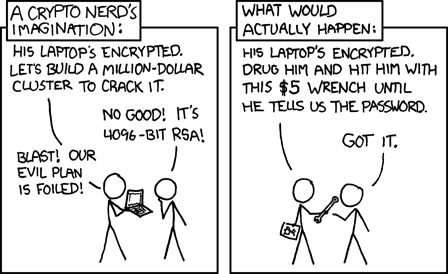
\includegraphics[width=10cm]{security.png}
        \else
            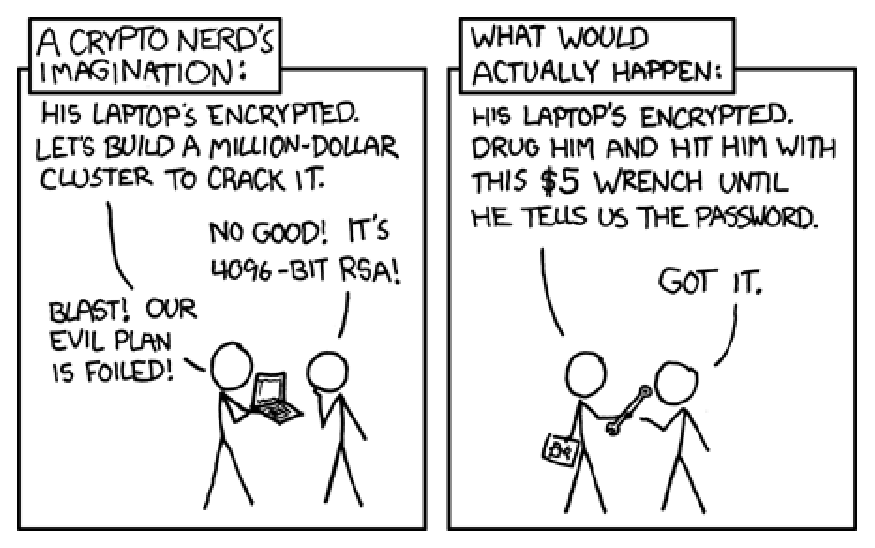
\includegraphics[width=10cm]{security.eps}
        \fi

        \url{http://xkcd.com/538/}. Ce dessin est publié sous licence \href{http://creativecommons.org/licenses/by-nc/2.5/}{ Creative Commons Attribution-NonCommercial 2.5 License}.
\end{center}

\noindent \ldots tout dépends du contexte.

%+++++++++++++++++++++++++++++++++++++++++++++++++++++++++++++++++++++++++++++++++++++++++++++++++++++++++++++++++++++++++++
\section{Représentations et caractères}
%+++++++++++++++++++++++++++++++++++++++++++++++++++++++++++++++++++++++++++++++++++++++++++++++++++++++++++++++++++++++++++

Une représentation est \defe{fidèle}{représentation!fidèle} si elle est injective en tant que application \( G\to \GL(V)\). Ce ne sont pas chacun des \( \rho(g)\) qui doivent être injectifs. La dimension de \( V\) est le \defe{degré}{degré!d'une représentation} de la représentation \( (V,\rho)\).

Si \( G\) est un groupe, l'ensemble des homomorphismes \( \Hom(G,\eC^*)\) est un groupe pour la multiplication. Un élément de \( \Hom(G,\eC^*)\) est un \defe{caractère abélien}{caractère!abélien}. Le nom «abélien» vient du fait que le caractère prenne ses valeurs dans \( \eC^*\). Nous notons \( \hat G=\Hom(G,\eC^*)\)\nomenclature[R]{\( \hat G\)}{groupe des caractères de \( G\)}.

\begin{theorem}
    Soit \( G\) un groupe abélien fini. Alors \( G\) est isomorphe à \( \hat G\).
\end{theorem}
L'isomorphisme n'est pas canonique.

\begin{proof}
    Étant donné la structure des groupes abéliens finis donnée par le théorème \ref{ThoRJWVJd}, nous commençons par nous concentrer sur \( G=\eZ/n\eZ\). Nous allons montrer que
    \begin{equation}
        \Hom(\eZ/n\eZ)\simeq \gU_n=\{ \xi\in \eC\tq \xi^n=1 \}.
    \end{equation}
    Pour cela nous avons l'isomorphisme
    \begin{equation}
        \begin{aligned}
            \psi\colon \Hom(\eZ,\eC^*)&\to \eC^* \\
            f&\mapsto f(1). 
        \end{aligned}
    \end{equation}
    Notons que si \( f\in \Hom(\eZ,\eC^*)\), alors \( f(k)=f(1)^k\), donc \( \psi\) est bien un isomorphisme. Cela nous amène à définir
    \begin{equation}
        \begin{aligned}
            \varphi\colon \Hom\Big( (\eZ/n\eZ,+),(\eC^*n\cdot) \Big)&\to \gU_n \\
            g&\mapsto f(1). 
        \end{aligned}
    \end{equation}
    Remarquons que pour tout \( f\in\Hom(\eZ/n\eZ,\eC^*)\) on a bien \( f(1)^n=1\). En effet si \( [k]\in \eZ/n\eZ\), alors \( f\big( [k] \big)=f(1)^k\) et en particulier
    \begin{equation}
        f(1)^n=f([n])=f(0)=1.
    \end{equation}
    Donc \( f(1)\in \gU_n\). Le \( \varphi\) est injective parce que si \( f(1)=g(1)\) alors \( f=g\) du fait que \( f(k)=f(1)^k=g(1)^k=g(k)\).

    Nous en sommes à avoir prouvé que \( \hat{\eZ/n\eZ}\simeq \gU_n\). Il faudrait encore montrer que \( \gU_n\simeq \eZ/n\eZ\). Pour cela nous nous rappelons de la sous-section \ref{SubSechZeTuL} nous ayant raconté que le groupe \( \gU_n\) des racines de l'unité était cyclique et d'ordre \( n\). Il est donc bien isomorphe à \( \eZ/n\eZ\).

    Passons au cas où
    \begin{equation}
        G\simeq \eZ/d_1\eZ\times \eZ/d_2\eZ\times \ldots\times \eZ/n_k\eZ.
    \end{equation}
    Dans ce cas nous montrons que 
    \begin{equation}
        \begin{aligned}
            \alpha\colon \bigtimes_{i=1}^k\Hom(\eZ/d_i\eZ,\eC^*)&\to \Hom(G,\eC^*) \\
            \alpha(\chi_1,\ldots, \chi_k)(g_1,\ldots, g_k)&= \chi_1(g_1)\ldots\chi_k(g_k). 
        \end{aligned}
    \end{equation}
    Ce \( \alpha\) est injectif parce qu'en appliquant l'égalité
    \begin{equation}
        \alpha(\chi_1,\ldots, \chi_k)=\alpha(\chi'_1,\ldots, \chi'_k)
    \end{equation}
    à l'élément \( g=(9,\ldots, 1,\ldots, 0)\) alors nous trouvons \( \chi_i(1)=\chi_i'(1)\) parce que \( \chi_j(0)=1\). Du coup \( \chi_i=\chi'_i\).

    L'application \( \alpha\) est en plus surjective. En effet si \( \chi\in\Hom(G,\eC^*)\), alors nous définissons
    \begin{equation}
        \chi_i(g_i)=\chi(0,\ldots, g_i,\ldots, 0),
    \end{equation}
    et nous avons alors \( \alpha(\chi_1,\ldots, \chi_k)=\chi\).

    Nous devons encore montrer que \( \alpha\) est un homomorphisme. Si \( \chi,\chi'\in\bigtimes_{i=1}^k\Hom(\eF_{d_i},\eC^*)\), alors
    \begin{subequations}
        \begin{align}
            \alpha(\chi\chi')(g_1,\ldots, g_k)&=(\chi_1\chi'_1)(g_1)\ldots (\chi_k\chi_k')(g_k)\\
            &=\chi_1(g_1)\ldots \chi_k(g_k)\chi'_1(g_1)\ldots \chi_k'(g_k)\\
            &=\alpha(\chi)(g_1,\ldots, g_k)\alpha(\chi')(g_1,\ldots, g_k)\\
            &=\big( \alpha(\chi)\alpha(\chi') \big)(g_1,\ldots, g_k).
        \end{align}
    \end{subequations}
    Donc \( \alpha(\chi\chi')=\alpha(\chi)\alpha(\chi')\).
\end{proof}

\begin{theorem}
    Soit \( G\) un groupe abélien fini. Les groupes \( G\) et \( \hat{\hat G}\) sont isomorphes et un isomorphisme canonique est donné par \( \alpha\colon g\mapsto f_g\) donné par
    \begin{equation}
        f_g(\chi)=\chi(g).
    \end{equation}
\end{theorem}

\begin{proof}

    D'abord \( f_g\) est bien un caractère de \( \hat G\) parce que
    \begin{equation}
        f_g(\chi\chi')=(\chi\chi')(g)=\chi(g)\chi'(g)=f_g(\chi)f_g(\chi').
    \end{equation}
    Le fait que \( \alpha\) soit un homomorphisme de groupes est direct :
    \begin{equation}
        f_{gg'}(\chi)=\chi(gg')=\chi(g)\chi(g')=f_g(\chi)f_{g'}(\chi)=(f_gf_{g'})(\chi).
    \end{equation}

    D'autre part nous savon que \( G\) et \( \hat{\hat G}\) ont le même cardinal. Il suffit donc de prouver l'injectivité de \( \alpha\) pour être sûr de la bijectivité. Pour cela nous devons prouver que si \( g\neq e\) alors \( f_g\neq f_e\). Nous savons que pour tout caractère \( \chi\in \hat G\), \( f_e(\chi)=\chi(e)=1\). Donc pour tout \( g\in G\setminus\{ e \}\), nous devons trouver \( \chi\in \hat G\) tel que \( \chi(g)\neq 1\).

    En vertu de ce que nous connaissons sur la structure des groupes abéliens finis (théorème \ref{ThoRJWVJd}), nous commençons \( G=\eZ/n\eZ\) et considérons le caractère donné par \( \chi([1])= e^{2i\pi/n}\). Ce \( \chi\) est un isomorphisme entre \( G\) et \( \gU(n)\); nous n'avons \( \chi([k])=0\) que si \( [k]=[n]=[0]\). Pour rappel dans \( \eZ/n\eZ\), le neutre est \( e=0\) et non \( e=1\).

    Passons au cas général :
    \begin{equation}
        G\simeq \eZ/n_1\eZ\times \ldots\times \eZ/n_k\eZ
    \end{equation}
    Si \( g=(g_1,\ldots, g_k)\) est non nul dans \( G\), alors il existe \( i\) tel que \( g_i\neq 0\) et on prend
    \begin{equation}
        \chi(g_1,\ldots, g_k)=\chi_i(g_i)
    \end{equation}
    où \( \chi_i\) est le caractère \( \chi_i([1])= e^{2\pi i/n_i}\). Ce \( \chi\) est alors un caractère non trivial de \( G\).
    
\end{proof}

%---------------------------------------------------------------------------------------------------------------------------
\subsection{Crochet de dualité et transformée de Fourier}
%---------------------------------------------------------------------------------------------------------------------------

Si \( G\) est un groupe abélien, nous définissons le crochet de dualité entre \( G\) et \( \hat G\) par
\begin{equation}
    \begin{aligned}
        \langle ., .\rangle \colon G\times \hat G&\to \eC^* \\
        \langle g, \chi\rangle &=\chi(g). 
    \end{aligned}
\end{equation}
Notons que l'image de ce crochet n'est pas \( \eC^*\) entier, mais seulement le groupe unitaire \( \gU(n)\) où \( n\) est l'exposant\footnote{Définition \ref{DefvtSAyb}.} de \( G\).


Si \( f,g\) sont des applications de \( G\) dans \( \eC\), alors on leur associe le produit scalaire
\begin{equation}
    \langle f, g\rangle =\frac{1}{ | G | }\sum_{s\in G}f(s)\overline{ g(s) }.
\end{equation}

\begin{lemma}
    Les caractères de \( G\) forment une base orthonormée de \( \eC^G\) pour ce produit scalaire.    
\end{lemma}

\begin{proof}
    Étant donné que les \( \chi(s)\) sont des nombres complexe de module \( 1\), nous avons \( \chi(s)\overline{ \chi(s) }=1\) et par conséquent \( \langle \chi, \chi\rangle =1\).

    Si par contre \( \chi\neq\chi'\), alors il existe \( s_\in G\) tel que \( \chi(s_0)\neq \chi'(s_0)\). Dans ce cas en effectuant un changement de variable \( s\to s_0s\) dans la sommation,
    \begin{subequations}
        \begin{align}
            \langle \chi, \chi'\rangle &=\frac{1}{ | G | }\sum_{s\in G}\chi(s)\overline{ \chi'(s) }\\
            &=\frac{1}{ | G | }\sum_{s\in G}\chi(s_0s)\overline{ \chi'(s_0s) }\\
            &=\frac{1}{ | G | }\chi(s_0)\chi'(s_0)\sum_{s\in G}\chi(s)\overline{ \chi'(s) }.
        \end{align}
    \end{subequations}
    Donc nous avons trouvé
    \begin{equation}
        \langle \chi, \chi'\rangle \big( 1-\chi(s_0)\overline{ \chi'(s_0) } \big)=0.
    \end{equation}
    Mais vu que \( \chi(s_0)\neq \chi(s'_0)\), la parenthèse est non nulle (pour rappel \( \chi(s_0)\) est un complexe de module \( 1\)) et par conséquent \( \langle \chi, \chi'\rangle =0\).

    Nous déduisons immédiatement que les caractères forment une famille libre parce que si \( \sum_i\chi_i=0\) (la somme est sur tous les caractères), alors en prenant le produit scalaire avec \( \chi_k\),
    \begin{equation}
        \sum_ia_i\langle \chi_k, \chi_i\rangle =0,
    \end{equation}
    et donc \( a_k=0\).

    Les caractères forment donc un système libre orthonormé. De plus l'espace engendré à la bonne dimension parce que le cardinal de l'ensemble des caractères est la dimension (complexe) de l'espace des fonction de \( G\) dans \( \eC\) parce que, en utilisant l'isomorphisme entre \( G\) et \( \hat G\),
    \begin{equation}
        \Card\hat G=\Card(G)=\dim_{\eC}\eC^G.
    \end{equation}
    La première 
\end{proof}

Du fait que les caractères forment une base orthonormée, nous pouvons écrire, pour toute application \( f\colon G\to \eC\),
\begin{equation}    \label{EqnnsXWC}
    f=\sum_{\chi\in\hat G}\langle \chi, f\rangle \chi.
\end{equation}
À une fonction \( f\colon G\to \eC\) nous associons la \defe{transformée de Fourier}{transformée!de Fourier!groupe abélien fini}\index{Fourier!transformée!groupe abélien fini}
\begin{equation}
    \begin{aligned}
        \hat f\colon \hat G&\to \eC \\
        \chi&\mapsto \langle \chi, f\rangle . 
    \end{aligned}
\end{equation}
Nous avons donc aussi une espèce de formule d'inversion
\begin{equation}
    f=\sum_{\chi\in\hat G}\hat f(\chi)\chi
\end{equation}
qui n'est qu'une réécriture de \ref{EqnnsXWC}.

%---------------------------------------------------------------------------------------------------------------------------
\subsection{Groupes non abéliens}
%---------------------------------------------------------------------------------------------------------------------------

Nous avons vu que le groupe des caractères \( \hat G\) contenait toute l'information sur un groupe abélien. Malheureusement, pour les groupes non abéliens, ça ne va pas suffire, et nous allons introduire la notion de représentations, dont les caractères seront un cas particulier de dimension un.

\begin{proposition}
    Soit \( G\) un groupe (pas spécialement abélien). Nous avons
    \begin{equation}
        \hat G\simeq\Hom\big( G/D(G),\eC^* \big).
    \end{equation}
\end{proposition}

\begin{proof}
    Ce qui fait fonctionner la preuve est le fait que si \( f\colon G\to \eC^*\) est un homomorphisme, alors \( f\) s'annule sur \( D(G)\). L'isomorphisme est
    \begin{equation}
        \begin{aligned}
            \psi\colon \hat G&\to \Hom\big( G/D(G),\eC^* \big) \\
            \psi(f)[g]&=f(g). 
        \end{aligned}
    \end{equation}
    Cette application est bien définie parce que si \( f\) est un homomorphisme,
    \begin{equation}
        f(gklk^{-1}l^{-1})=f(g).
    \end{equation}
    D'autre part \( \psi\) est un homomorphisme de groupe parce que
    \begin{equation}
        \psi(f_1f_2)[g]=(f_1f_2)(g)=f_1(g)f_2(g)=\psi(f_1)[g]\psi(f_2)[g]=\big( \psi(f_1)\psi(f_2) \big)[g].
    \end{equation}
    Pour l'injectivité de \( \psi\), soit \( f_1\) et \( f_2\) telles que \( \psi(f_1)=\psi(f_2)\). Alors pour tout \( g\in G\) nous avons
    \begin{equation}
        \psi(f_1)[g]=\psi(f_2)[g]
    \end{equation}
    et donc \( f_1(g)=f_2(g)\).

    Enfin \( \psi\) est surjective. En effet, soit \( \bar f\in\Hom\big( G/D(G),\eC^* \big)\). Alors nous obtenons \( \psi(f)=\bar f\) en posant
    \begin{equation}
        f(g)=\bar f[g].
    \end{equation}
    Il faut juste vérifier que le \( f\) ainsi défini est dans \( \hat G\), c'est à dire que \( f(g_1g_2)=f(g_1)f(g_2)\).
\end{proof}

Cette proposition nous montre que
\begin{equation}
    \hat G=\widehat{G/D(G)},
\end{equation}
alors que \( G/D(G)\) est abélien; il n'est donc pas tellement possible que \( \hat G\) contienne beaucoup d'informations intéressantes sur \( G\).

%---------------------------------------------------------------------------------------------------------------------------
\subsection{Représentations linéaires des groupes finis}
%---------------------------------------------------------------------------------------------------------------------------

Soit \( V\), un \( \eC\)-espace vectoriel de dimension finie. Une \defe{représentation}{représentation} linéaire de \( G\) dans \( V\) est un homomorphisme \( \rho\colon G\to \End(V)\). Nous notons \( (V,\rho)\) cette représentation. Voire \( \rho\) tout court si l'espace vectoriel n'est pas ambigu.

Si \( \dim V=1\), alors \( \GL(V)=\eC^*\) et les représentation sont les caractères abéliens.

\begin{example} \label{ExKUAyUD}
    Considérons le triangle équilatéral \( A,B,C\), par exemple donné par les points
    \begin{subequations}
        \begin{numcases}{}
            A=1\\
            B=(-\frac{ 1 }{2},\frac{ \sqrt{3} }{2})\\
            C=(-\frac{ 1 }{2},-\frac{ \sqrt{3} }{2})\\
        \end{numcases}
    \end{subequations}
    Dans la base (pas orthonormée) \( \{ A,B \}\) de \( \eR^2\), ces trois points sont donnés par
    \begin{equation}
        \begin{aligned}[]
            A&=\begin{pmatrix}
                1    \\ 
                0    
            \end{pmatrix}&B&=\begin{pmatrix}
                0    \\ 
                1    
            \end{pmatrix}&C&=\begin{pmatrix}
                -1    \\ 
                -1    
            \end{pmatrix}.
        \end{aligned}
    \end{equation}
    Le groupe symétrique\index{groupe!symétrique!action sur un triangle} \( S_3\) agit sur le triangle par permutation des sommets. Vues dans la base \( \{ A,B \}\), les transpositions correspondent aux matrices
    \begin{subequations}
        \begin{align}
            (A,B)&\to\begin{pmatrix}
                0    &   1    \\ 
                1    &   0    
            \end{pmatrix}\\
            (A,C)&\to \begin{pmatrix}
                -1    &   0    \\ 
                -1    &   1    
            \end{pmatrix}\\
            (B,C)&\to\begin{pmatrix}
                1    &   -1    \\ 
                0    &   -1    
            \end{pmatrix}.
        \end{align}
    \end{subequations}
    La permutation \( (A,B,C)\) s'écrit comme \( (A,B,C)=(A,C)(A,B)\) et on lui associe la matrice
    \begin{equation}
        (A,B,C)\to\begin{pmatrix}
            0    &   -1    \\ 
            1    &   -1    
        \end{pmatrix}.
    \end{equation}
    C'est bien le produit des matrices de \( (A,C)\) et de \( (A,B)\). De la même façon nous avons
    \begin{equation}
        (BAC)<++>
    \end{equation}
    % TODO : il y a manifestement quelque chose à terminer ici.
    <++>
\end{example}

Si \( (V,\rho)\) et \( (V',\rho')\) sont deux représentations du groupe \( G\), alors nous définissons la \defe{somme directe}{somme directe (de représentations)} par \( \big( V\oplus V',\rho\oplus\rho' \big)\) donné par
\begin{equation}
    (\rho\oplus\rho')(g)=\begin{pmatrix}
        \rho(g)    &   0    \\ 
        0    &   \rho'(g)    
    \end{pmatrix}\in \GL(V\oplus V').
\end{equation}

Nous noterons souvent \( 2V\) pour la représentations \( (V,\rho)\oplus (V,\rho)\) et plus généralement l'écriture
\begin{equation}
    V=\bigoplus_i k_iW_i
\end{equation}
signifiera la représentation somme de \( k_i\) termes de la représentation \( W_i\). Ici encore un abus est commis entre la représentation \( (\rho_i,W_i)\) et l'espace \( W_i\).

%---------------------------------------------------------------------------------------------------------------------------
\subsection{Module}
%---------------------------------------------------------------------------------------------------------------------------

Nous considérons la \( \eC\)-algèbre \( G[\eC]\)\nomenclature[G]{\( \eC[G]\)}{combinaisons d'éléments de \( G\) à coefficients dans \( \eC\)} des combinaisons (formelles) d'éléments de \( G\) à coefficients dans \( G\), c'est à dire l'ensemble
\begin{equation}
    \eC[G]=\{ \sum_{s\in G}a_ss \}
\end{equation}
avec le produit hérité de la bilinéarité :
\begin{equation}
    \sum_{s\in G}\sum_{t\in G}a_sb_tst=\sum_s\sum_t a_sb_{s^{-1}t}t,
\end{equation}
et la somme
\begin{equation}
    (\sum_sa_ss)+\sum_tb_tt=\sum_{s\in G}(a_s+b_s)s.
\end{equation}
Le tout est une \( \eC\)-algèbre agissant sur \( V\) par
\begin{equation}
    \left( \sum_sa_ss \right)v=\sum_{s\in G}a_s\rho(s)v\in V
\end{equation}

Les sous-modules indécomposables seront les représentations irréductibles.

\begin{definition}
    La représentation \( (V,\rho)\) du groupe \( G\) est \defe{irréductible}{irréductible!représentation}\index{représentation!irréductible} si les seuls sous-espaces invariants de \( V\) sous \( \rho(G)\) sont $V$ et \( \{ 0 \}\).
\end{definition}

\begin{example}
    La représentation de \( S_3\) sur \( \eR^2\) donnée par les permutations des sommets d'un triangle équilatéral donnée dans l'exemple \ref{ExKUAyUD} est irréductible.
\end{example}

La question qui vient est de savoir si une représentation possédant des sous-espaces invariants peut être écrite comme la somme de représentations irréductibles.

\begin{proposition} \label{PropHeyoAN}  \index{représentation!irréductible}
    Soit \( (V,\rho)\) une représentation linéaire de dimension finie d'un groupe fini\footnote{La démonstration marche aussi pour les groupes compacts, mais il faudrait des intégrales.}. Si \( W_1\) est un sous-espace stable\footnote{c'est à dire si \( \rho\) n'est pas irréductible.}, alors il existe un sous-espace \( W_2\) également stable et tel que \( V=W_1\oplus W_2\).

    Toute représentation linéaire est décomposable en représentations irréductibles.
\end{proposition}

\begin{proof}
    Soit \( P\colon V\to V\) un projecteur sur \( W_1\), c'est à dire que \( P^2=P\) et \( P(V)=W_1\). Pour construire un tel projecteur, on peut par exemple prendre un supplémentaire de \( W_1\) dans \( V\) puis utiliser la décomposition\footnote{Ou encore prendre une base de \( W_1\), l'étendre en une base de \( V\) et définir \( P\) comme l'annulation des coefficients des vecteurs «complétant» la base.}. Nous considérons l'opérateur
    \begin{equation}
        P_G=\frac{1}{ | G | }\sum_{g\in G}\rho(g)\circ P\circ \rho(g)^{-1}.
    \end{equation}
    Prouvons que ce \( P_G\) est encore un projecteur. D'abord pour tout \( g\in G\) nous avons
    \begin{equation}
        \rho(g)P_G\rho(g)^{-1}=\frac{1}{ | G | }\sum_{s\in G}\rho(gs)P\rho(gs)^{-1}=P_G.
    \end{equation}
    La dernière égalité est un changement de variables dans la somme\footnote{Et c'est ça qui demande un peu de technique pour écrire la preuve dans le cas d'un groupe compact : il faut une mesure de Haar.}. Cela signifie que \( P_G\rho=\rho P_G\). Nous avons même \( P_GP=P\) parce que si \( v\in W_1\), alors 
    \begin{subequations}
        \begin{align}
            P_G(v)&=\frac{1}{ | G | }\sum_{s\in G}\rho(s)P\underbrace{\rho(s)^{-1} v}_{\in W_1}\\
            &=\frac{1}{ | G | }\sum_s\rho(s)\rho(s)^{-1} v\\
            &=v.
        \end{align}
    \end{subequations}
    Avec cela nous pouvons conclure que \( P_G^2=P_G\) parce que
    \begin{subequations}
        \begin{align}
            P_G\circ P_G&=\frac{1}{ | G | }\sum_g P_G\rho(g)P\rho(g)^{-1}\\
            &=\frac{1}{ | G | }\sum_g \rho(g)P_GP\rho(g)^{-1}\\
            &=\frac{1}{ | G | }\sum_g \rho(g)P\rho(g)^{-1}\\
            &=P_G.
        \end{align}
    \end{subequations}
    Donc \( P_G\) est un projecteur, est stable sous les conjugaisons par \( \rho(g)\) et commute avec \( \rho(g)\). Nous décomposant \( \id\) de façon évidente en
    \begin{equation}
        \id=P_G+(\id-P_G).
    \end{equation}
    Étant donné que l'opérateur \( P_G\) commute avec tous les \( \rho(g)\), les noyaux de \( P_G\) et \( \id-P_G\) sont des sous-espaces invariants. Vu que \( P_G\) est un projecteur, nous avons \( q(P_G)=0\) avec \( q(X)=X^2-X\). Pour appliquer le lemme des noyaux (théorème \ref{ThoDecompNoyayzzMWod}), nous remarquons que \( q(X)=X(X-1)\) et donc 
    \begin{equation}
        V=\ker P_G\oplus\ker(P_G-\mtu).
    \end{equation}
    Si nous posons \( W_2=\ker P_G\), il reste à voir que \( \ker(P_G\mtu)=W_1\). D'abord \( W_1\subset\ker(P_G-\id)\) parce que si \( w\in W_1\), ce dernier étant stable,
    \begin{subequations}
        \begin{align}
            P_Gw&=\frac{1}{ | G | }\sum_{g\in G}\rho(g)P\underbrace{\rho(g)^{-1}w}_{\in W_1}\\
            &=\frac{1}{ | G | }\sum_{g\in G}w\\
            &=w.
        \end{align}
    \end{subequations}
    Pour prouver l'inclusion inverse, nous savons que \( P_G\) et \( P\) sont des projecteurs tels que \( P_GP=P\), ce qui signifie que l'image de \( P_G\) est inclue à celle de \( P\), c'est à dire à \( W_1\). Mais \( \Image(P_G)=\ker(\mtu-P_G)\), donc
    \begin{equation}
        \ker(\mtu-P_G)=\Image(P_G)\subset\Image(P)=W_1.
    \end{equation}

    La représentation \( \rho\) se décompose donc en deux sous-représentations \( (\rho,W_1)\) et \( \rho,W_2\). Si l'une des deux n'est pas irréductible, le processus peut recommencer. Vu que la dimension de \( V\) est finie, toute représentation se décompose en une somme finie de représentation irréductibles.
\end{proof}

%---------------------------------------------------------------------------------------------------------------------------
\subsection{Structure hermitienne}
%---------------------------------------------------------------------------------------------------------------------------

Soit \( (\rho,V)\) une représentation de \( G\) sur un espace vectoriel complexe \( V\). Nous voulons munir \( V\) d'un produit scalaire hermitien (définition \ref{DefMZQxmQ}) tel que les opérateurs \( \rho(g)\) soient tous des isométries. C'est à dire que nous voudrions définir \( \langle u, v\rangle_G\) de telle sorte à avoir
\begin{equation}
    \langle \rho(g)u, \rho(g)v\rangle_G =\langle u, v\rangle_G
\end{equation}
pour tout \( g\in G\). Nous commençons par considérer un produit hermitien \( \langle ., .\rangle \) quelconque et puis nous définissons
\begin{equation}
    \langle u, v\rangle_G=\frac{1}{ | G | }\sum_{g\in G}\langle \rho(g)u, \rho(g)v\rangle.
\end{equation}
Nous devons vérifier que c'est un produit. La seule des conditions dont la vérification n'est pas immédiate est celle de positivité. Pour tout \( g\in G\) et tout \( v\in V\), nous avons \( \langle \rho(g)v, \rho(g)v\rangle \) est positif et nul si et seulement si \( \rho(g)v=0\). Étant donné que \( \rho(e)v=v\), parmi les termes de la somme
\begin{equation}
    \langle u, u\rangle_G=\frac{1}{ | G | }\sum_{g\in G}\langle \rho(g)v, \rho(g)v\rangle,
\end{equation}
au moins un est strictement positif (pourvu que \( v\neq 0\)); les autres sont positifs ou nuls. Par conséquent \( \langle v, v\rangle_G=0\) si et seulement si \( v=0\).

Donc les groupes finis peuvent être vus comme des parties de groupes d'isométrie. De la même façon, en utilisant une mesure de Haar pour faire la moyenne, nous pouvons plonger les groupes compacts dans des groupes unitaires.

%---------------------------------------------------------------------------------------------------------------------------
\subsection{Caractères}
%---------------------------------------------------------------------------------------------------------------------------

Soit \( (V,\rho)\) une représentation linéaire du groupe \( G\). Le \defe{caractère}{caractère} de \( \rho\) est la fonction
\begin{equation}
    \begin{aligned}
        \chi_{\rho}\colon G&\to \eC \\
        s&\mapsto \tr\big( \rho(s) \big).
    \end{aligned}
\end{equation}
Par invariance de la trace, nous avons
\begin{equation}
    \chi_{\rho}(sts^{-1})=\chi_{\rho}(t),
\end{equation}
ce qui fait que le caractère est une fonction constante sur les classes de conjugaison.

Un \defe{caractère irréductible}{caractère!irréductible} est un caractère d'une représentation irréductible.

\begin{definition}
    Une application \( f\colon G\to \eC\) est \defe{centrale}{centrale (application)} si elle est constante sur les classes de conjugaison.
\end{definition}
Les traces sont des applications centrales.

L'ensemble des fonctions centrales sur un groupe fini (ou tout au moins ayant un nombre fini de classes de conjugaison) est un \( \eC\)-espace vectoriel de dimension égale au nombre de classes, et nous pouvons mettre le produit scalaire
\begin{equation}    \label{EqJrEpVI}
    \langle f, g\rangle =\frac{1}{ | G | }\sum_{s\in G}f(s)\overline{ g(s) }.
\end{equation}
C'est une forme hermitienne sur l'espace des fonction centrales.

%+++++++++++++++++++++++++++++++++++++++++++++++++++++++++++++++++++++++++++++++++++++++++++++++++++++++++++++++++++++++++++
\section{Équivalence de représentations et caractères}
%+++++++++++++++++++++++++++++++++++++++++++++++++++++++++++++++++++++++++++++++++++++++++++++++++++++++++++++++++++++++++++

Cette section prend des éléments des articles \wikipedia{fr}{Lemme_de_Schur}{lemme de Schur}, \wikipedia{fr}{Caractère_d'une_représentation_d'un_groupe_fini}{caractère d'une représentation}, \wikipedia{fr}{Fonction_centrale_d'un_groupe_fini}{fonction centrale} et \wikipedia{fr}{Trace_(algèbre)}{trace} de wikipédia.

Nous disons que les deux représentations \( (V,\rho)\) et \( (V',\rho')\) sont \defe{équivalentes}{equivalence@équivalence!de représentations} si il existe une bijection linéaire \( f\colon V\to V'\) telle que
\begin{equation}
    f\circ \rho=\rho'\circ f.
\end{equation}
Nous disons alors que \( f\) \defe{entrelace}{entrelacement} \( \rho\) et \( \rho'\).

\begin{theorem}[Théorème de Schur]\index{théorème!Schur}\index{Schur (théorème)}    \label{ThoyftobH}
    Si \( (V,\rho)\) et \( (V',\rho')\) sont des représentations irréductibles non équivalentes alors la seule application linéaire \( f\colon V\to V'\) entrelaçant \( \rho\) et \( \rho'\) est la fonction nulle.

    En d'autres termes, soit les représentations sont équivalentes (et il y a un isomorphisme), soit il n'y a même pas un homomorphisme.
\end{theorem}

\begin{proof}
    Soit \( f\in\aL(V,V')\) telle que \( f\circ \rho=\rho'\circ f\). Alors \( \ker f\) est un sous-espace stable sous \( \rho(G)\), et \( \Image(f)\) est un sous-espace de \( V'\) stable par \( \rho'(G)\). Par irréductibilité, nous avons que \( \ker(f)=\{ 0 \}\) ou \( V\). Même chose pour \( \Image(f)\). Il y a deux possibilités.
    \begin{enumerate}
        \item
            Si \( \ker(f)=\{ 0 \}\), alors \( \Image(f)\neq \{ 0 \}\) et alors \( \Image(f)=V'\). Du coup \( f\) est injective et surjective, c'est à dire est un isomorphisme.
        \item
            Si \( \ker(f)=V\), alors \( f=0\).
    \end{enumerate}
\end{proof}

\begin{corollary}[Schur pour les représentations sur \( \eC\)]
    Soit \( (V,\rho)\) une représentation irréductible, alors l'ensemble
    \begin{equation}
        \End_{G}(V,\rho)=\{ f\in\End(V)\tq \rho\circ f=f\circ \rho \}
    \end{equation}
    est l'ensemble des homothéties.
\end{corollary}

\begin{proof}
    Soit \( f\in\End_{G}(V,\rho)\). Vu que l'espace est sur \( \eC\), l'endomorphisme \( f\) a une valeur propre \( \lambda\). L'opérateur \( g=f-\lambda\mtu\) est aussi un opérateur d'entrelacement de \( \rho\) alors que \( \ker(g)\neq \{ 0 \}\) par définition de valeur propre. Du coup \( \ker(g)=V\), ce qui signifie que \( f\) est l'isométrie de rapport \( \lambda\) : \( f=\lambda\id\).
\end{proof}

\begin{lemma}   \label{LempUSOlo}
    Si \( (\rho,V)\) et \( (\rho',V')\) sont des représentations équivalentes de caractères \( \chi\) et \( \chi'\), alors \( \chi=\chi'\).
\end{lemma}

\begin{proof}
    Si \( A\colon V\to V'\) est un isomorphisme d'espace vectoriel entrelaçant \( \rho\) et \( \rho'\), c'est à dire si pour tout \( g\), \( \rho'(g)A=A\rho(g)\), alors \( \rho'(g)=A\rho(g)A^{-1}\) et
    \begin{equation}
        \chi'(g)=\tr\big( \rho'(g) \big)=\tr\big( A\rho(g)A^{-1} \big)=\tr\big( \rho(g) \big)
    \end{equation}
    parce que la trace est un invariant de similitude (lemme \ref{LemhbZTay}).
\end{proof}

\begin{lemma}   \label{LemJqIZns}
    Si \( \chi\) est le caractère de la représentation complexe \( (V,\rho)\) du groupe fini \( G\), alors pour tout \( g\in G\) nous avons \( \chi(g^{-1})=\overline{ \chi(g) }\).
\end{lemma}

\begin{proof}
    Par le corollaire \ref{CorpZItFX} au théorème de Lagrange, nous avons \( g^{| G |}=e\) et donc en tant qu'opérateur, \( \rho(g)^{| G |}=\mtu\). Les valeurs propres de \( \rho(g)\) sont donc des racines de l'unité. Si nous notons \( \lambda_i\) ces valeurs propres, alors \( \chi(g)=\sum_i\lambda_i\), et en considérant la matrice dans sa base de diagonalisation (lemme de Schur complexe, \ref{LemSchurComplHAftTq}), nous voyons que
    \begin{equation}
        \chi(g^{-1})=\tr\big( \rho(g)^{-1} \big)=\sum_i\frac{1}{ \lambda_i }.
    \end{equation}
    Mais \( \lambda_i\) étant une racine de l'unité nous avons \( \frac{1}{ \lambda_i }=\bar\lambda_i\), ce qui fait que
    \begin{equation}
        \chi(g^{-1})=\sum_i\bar\lambda_i=\overline{ \chi(g) }.
    \end{equation}
\end{proof}

\begin{proposition} \label{PropJzbfWi}
    Soient deux représentations irréductibles complexes \( (V,\rho)\) et \( (V',\rho')\) du même groupe fini \( G\), et \( \chi\) et \( \chi'\) leurs caractères respectifs. Nous avons
    \begin{enumerate}
        \item
            \( \langle \chi, \chi'\rangle =0\) si \( \rho\) et \( \rho'\) ne sont pas équivalentes.
        \item
            \( \langle \chi, \chi'\rangle =1\) si les représentations sont équivalentes.
    \end{enumerate}
\end{proposition}

\begin{proof}
    Nous considérons les bases \( \{ e_1,\ldots, e_n \} \) de \( V\) et \( \{ f_1,\ldots, f_m \}\) de \( V'\). Puis nous considérons la matrice $F(k,l)=E_{kl}\in\eM_{m,n}(\eC)$ où pour rappel, \( E_{kl}\) est la matrice de composantes \( (E_{kl})_{ij}=\delta_{ki}\delta_{lj}\). Nous posons
    \begin{equation}
        F_G(k,l)=\frac{1}{ | G | }\sum_{g\in G}\rho(g)\circ F(k,l)\circ\rho'(g)^{-1}.
    \end{equation}
    En nous permettant de ne pas réécrire les indices \( k\) et \(l \) de \( F\) et \( F_G\), nous montrons que \( F_G\) entrelace \( \rho\) et \( \rho'\) :
    \begin{subequations}
        \begin{align}
            F_G\circ\rho'(t)&=\frac{1}{ | G | }\sum_{s\in G}\rho(s)\circ F\circ \rho'(s^{-1})\circ \rho(t)\\
            &=\frac{1}{ | G | }\sum_s\rho(s)F\rho'(s^{-1} t)\\
            &=\frac{1}{ | G | }\sum_{k}\rho(tk)F\rho'(k^{-1})\\
            &=\frac{1}{ | G | }\rho(t) \sum_k\rho(k)F\rho'(k^{-1})\\
            &=\rho(t)\circ F_G.
        \end{align}
    \end{subequations}
    Dans ce calcul nous avons effectué le changement de variables \( k=(s^{-1} t)^{-1}\) qui donne \( s=tk\).

    Par ailleurs nous avons
    \begin{subequations}
        \begin{align}
            \Big( \rho(g)F(k,l)\rho'(g^{-1}) \Big)_{ij}&=\sum_{r=1}^n\sum_{s=1}^m\rho(g)_{ir}F(k,l)_{rs}\rho'(g^{-1})_{sj}\\
            &=\sum_{rs}\rho(g)_{ir}\delta_{kr}\delta_{ls}\rho'(g^{-1})_{sj}\\
            &=\rho(g)_{ik}\rho'(g^{-1})_{lj},
        \end{align}
    \end{subequations}
    et par conséquent
    \begin{equation}    \label{Eqgvpzfz}
        F_G(k,l)_{ij}=\frac{1}{ | G | }\sum_{g\in G}\rho(g)_{ik}\rho'(g^{-1})_{lj}.
    \end{equation}
    Si \( \chi\) et \( \chi'\) sont les caractères de \( \rho\) et \( \rho'\), alors nous avons le produit \eqref{EqJrEpVI} qui donne
    \begin{subequations}
        \begin{align}
            \langle \chi, \chi'\rangle &=\frac{1}{ | G | }\sum_{g\in G}\chi(g)\overline{ \chi'(g) }\\
            &=\frac{1}{ | G | }\sum_g\chi(g)\chi'(g^{-1})    &\text{lemme \ref{LemJqIZns}}\\
            &=\frac{1}{ | G | }\sum_g\sum_{i=1}^n\sum_{j=1}^m\rho(g)_{ii}\rho'(g^{-1})_{jj}     \label{sEqKYywTM}\\
            &=\sum_{ij}F_G(i,j)_{ij}    &\text{par \eqref{Eqgvpzfz}}.
        \end{align}
    \end{subequations}
    Si les représentations \( \rho\) et \( \rho'\) ne sont pas équivalentes, le fait que \( F_G\) en soit un opérateur d'entrelacement implique par le théorème de Schur \ref{ThoyftobH} que \( F_G=0\) et donc \( \langle \chi, \chi'\rangle =0\).

    Si au contraire les représentation sont équivalentes, alors le lemme \ref{LempUSOlo} nous dit que \( \chi=\chi'\) et nous reprenons la définition :
    \begin{equation}
        \langle \chi, \chi\rangle =\frac{1}{ | G | }\sum_g\chi(g)\overline{ \chi(g) }=\frac{1}{ | G | }\sum_{g\in G}1=1
    \end{equation}
    parce que les nombres \( \chi(g)\) sont des racines de l'unité.
\end{proof}


%--------------------------------------------------------------------------------------------------------------------------- 
\subsection{Représentation régulière}
%---------------------------------------------------------------------------------------------------------------------------

Nous notons \( \lambda\) la \defe{représentation régulière gauche}{représentation!régulière gauche}, agissant sur le \( \eK\)-espace vectoriel des fonctions \( G\to \eK\) par
\begin{equation}
    \Big( \lambda(g)f \Big)(g)=f(g^{-1}h).
\end{equation}
D'autre part nous considérons les fonction \( \delta_g\colon G\to \eK\) (ici \( \eK\) est \( \eR\) ou \( \eC\) ou pire) définie par
\begin{equation}
    \delta_g(h)=\begin{cases}
        1    &   \text{si \( g=h\)}\\
        0    &    \text{sinon.}
    \end{cases}
\end{equation}
La représentation régulière agit sur les fonctions \( \delta_s\) de la façon suivante :
\begin{equation}
    \lambda(g)\delta_s=\delta_{gs}
\end{equation}
parce que \( \big( \lambda(g)\delta_s \big)(h)=\delta_s(g^{-1}h)=\delta_{gs}(h)\).

\begin{lemma}
    Le caractère de la représentation régulière gauche est donné par 
    \begin{equation}        \label{EqUuoVNa}
        \chi_{\lambda}=| G |\delta_e.
    \end{equation}
\end{lemma}

\begin{proof}
    Appliquer l'équation \eqref{EqUuoVNa} fonctionne parce que \( \chi_{\lambda}(e)\) est la dimension de l'espace des fonctions sur \( G\), c'est à dire \( | G |\). Si par contre \( g\neq e\), alors \( \lambda(g)\) est une matrice de permutation (dans la base des \( \delta_h\)) et a donc tous ses éléments diagonaux nuls.
\end{proof}

Si \( \rho\) est une représentation et si \( f\) est une fonction sur le groupe, alors nous considérons l'opérateur
\begin{equation}
    \rho_f=\sum_{g\in G}f(g)\rho(g).
\end{equation}

\begin{proposition}[\cite{NhCRhg}]  \label{PropEAXkAY}
    Si \( (\rho,V)\) est une représentation irréductible et si \( f\) est une fonction centrale sur \( G\), alors l'opérateur \( \rho_f\) est une homothétie de \( V\) de rapport
    \begin{equation}
        \frac{1}{ \dim V }\sum_{g\in G}f(g)\chi(g)
    \end{equation}
    où \( \chi\) est le caractère de \( \rho\).
\end{proposition}

\begin{proof}
    Nous commençons par voir que \( \rho_f\) entrelace \( \rho\). En effet,
    \begin{subequations}
        \begin{align}
            \rho(t)^{-1}\circ\rho_f\circ\rho(t)&=\sum_gf(g)\rho(t^{-1}gt)\\
            &=\sum_hf(tht^{-1})\rho(g)      &\text{\( h=t^{-1}gt\)}\\
            &=\sum_hf(h)\rho(h)\\
            &=\rho_f
        \end{align}
    \end{subequations}
    où en écrivant \( f(tht^{-1})=f(h)\), nous avons utilisé le fait que \( f\) était centrale. Étant donné que \( \rho_f\) entrelace une représentation irréductible, le lemme de Schur (\ref{ThoyftobH}) nous indique que \( \rho_f\) est une homothétie. Soit \( k\) le facteur d'homothétie. Alors d'une part \( \tr(\rho_f)=nk\). D'autre part,
    \begin{subequations}
        \begin{align}
            \tr(\rho_f)&=\tr\big( \sum_gf(g)\rho(g) \big)\\
            &=\sum_gf(g)\tr\big( \rho(g) \big)\\
            &=\sum_gf(g)\chi(g).
        \end{align}
    \end{subequations}
    Du coup effectivement 
    \begin{equation}
        k=\frac{1}{ n }\sum_{g\in G}f(g)\chi(g).
    \end{equation}
\end{proof}

%--------------------------------------------------------------------------------------------------------------------------- 
\subsection{Caractères et représentations : suite et fin}
%---------------------------------------------------------------------------------------------------------------------------

\begin{lemma}
    Un groupe fini n'a (à équivalence près) qu'un nombre fini de représentations irréductibles.
\end{lemma}

\begin{proof}
    Les caractères irréductibles forment un système orthonormé (proposition \ref{PropJzbfWi}) et donc libre parmi les fonctions centrales. Donc il y a au plus autant de caractères irréductibles que la dimension de l'espace des fonctions centrales; et ce dernier est de dimension finie donnée par le nombre de classes de conjugaison de \( G\).
\end{proof}

Nous savons que les caractères de deux représentations irréductibles sont égaux. Étant donné qu'il n'existe qu'un nombre fini de représentations irréductibles, il existe un nombre fini de caractères irréductibles. Nous pouvons donc fixer les notations suivantes. Les caractères irréductibles seront notés \( \{ \varphi_i \}_{i=1,\ldots, h}\) et nous noterons \( (\sigma_i,W_i)\) une représentation ayant le caractère \( \varphi_i\).

\begin{theorem}[\cite{NhCRhg}]
    Soit \( (\rho,V)\) une représentation de \( G\) de caractère \( \chi\). Alors sa décomposition en représentations irréductibles est donnée par
    \begin{equation}
        (V,\rho)=\bigoplus_{i=1}^hk_i(W_i,\sigma_i)
    \end{equation}
    avec \( k_i=\langle \chi, \varphi_i\rangle \). En particulier, à permutation près des facteurs, la décomposition d'une représentation en représentations irréductibles est unique.
\end{theorem}

\begin{proof}
    La décomposition de \( \chi\) en caractères irréductibles est donnée par \( \chi=\sum_ik_i\varphi_i\); en prenant le produit de cette égalité avec \( \varphi_j\) et en tenant compte de l'othonormalité des caractères irréductibles,
    \begin{equation}
        \langle \chi, \varphi_j\rangle =\sum_ik_i\langle \varphi_i, \varphi_j\rangle =k_j.
    \end{equation}
\end{proof}

Le théorème suivant est ce qui nous permet de dire que l'étude des caractères et l'étude des représentations, c'est la même chose.

\begin{theorem} \label{ThoWGkfADd}
    Soit \( G\) un groupe fini\footnote{Nous sommes depuis longtemps dans l'étude des représentations des groupes finis.}.
    \begin{enumerate}
        \item   \label{ItemZReOWoHi}
            Deux représentations sont équivalentes si et seulement si elles ont même caractères.
        \item   \label{ItemZReOWoHii}
            Si \( \chi\) est un caractère, alors 
            \begin{enumerate}
                \item
                    \( \langle \chi, \chi\rangle \in \eN\) 
                \item
                    \( \langle \chi, \chi\rangle =1\) si et seulement si c'est un caractère irréductible.   
            \end{enumerate}
    \end{enumerate}
\end{theorem}

\begin{proof}
    Nous démontrons chaque point séparément.
    \begin{enumerate}
        \item
            
    Le fait que deux représentations équivalentes aient même caractère est le lemme \ref{LempUSOlo}. Nous montrons l'autre sens. Si \( (\rho,V)\) et \( (\rho',V')\) sont deux représentations irréductibles de décompositions
    \begin{subequations}
        \begin{align}
            V&=\bigoplus_ik_iW_i\\
            V'&=\bigoplus_ik_i'W_i,
        \end{align}
    \end{subequations}
    alors si \( \chi=\chi'\), nous avons \( k_i=k'_i\) et les représentations sont identiques.

\item

    Soit \( (\rho,V)\) une représentation ayant \( \chi\) comme caractère. En posant \( k_i=\langle \chi, \varphi_i\rangle \) nous avons la décomposition en représentations irréductibles
    \begin{equation}
        V=\bigoplus_ik_iW_i,
    \end{equation}
    et aussi
    \begin{equation}
        \langle \chi, \chi\rangle =\langle \sum_ik_i\varphi_i, \sum_jk_j\varphi_j\rangle =\sum_ik_i^2\in \eN.
    \end{equation}
    Ce nombre est de plus égal à \( 1\) si et seulement si tous les termes de la somme sont nuls sauf un qui vaudrait \( 1\). Ce cas donne une représentation irréductible.

    \end{enumerate}
    
\end{proof}

\begin{proposition} \label{PropYLnxIjk}
    Si \( (\lambda,R)\) est la représentation régulière gauche de décomposition en représentations irréductibles
    \begin{equation}
        R=\bigoplus_ik_iW_i,
    \end{equation}
    alors
    \begin{enumerate}
        \item
            \( k_i=\dim W_i\),
        \item
            \( \sum_i(\dim W_1)^2=|G|\),
        \item   \label{ItemEXAjTIh}
            pour tout \( g\in G\), \( \sum_i(\dim W_i)\varphi_i(g)=0\)\footnote{Cette propriété est appelée «orthogonalité des colonnes» pour une raison qui apparaîtra au moment de compléter le tableau \eqref{EqOKtZYFQ}.}.
        \item
            Une autre façon d'énoncer le résultat \ref{ItemEXAjTIh} est de dire que si \( \{ (n_i,\varphi_i) \}\) est la liste des couples dimension,caractère des représentations irréductibles non équivalentes, alors pour tout \( s\in G\setminus\{ e \}\) nous avons \( \sum_{i=1}^pn_i\varphi_i(s)=0\) où la somme porte sur les représentations irréductibles non équivalentes.
    \end{enumerate}
\end{proposition}

\begin{proof}
    Nous notons \( r\) le caractère de la représentation régulière gauche. Nous avons
    \begin{equation}
        k_i=\langle r, \varphi_i\rangle =\frac{1}{ | G | }\sum_{s\in G}r(s)\overline{ \varphi_i(s) }=\overline{ \varphi_i(e) }.
    \end{equation}
    Mais \( \varphi_i(e)=\dim W_i\in \eR\), donc nous avons bien \( k_i=\dim W_i\). Le caractère de la représentation régulière peut alors s'exprimer de deux façons :
    \begin{equation}
        | G |\delta_e=\sum_i(\dim W_i)\varphi_i.
    \end{equation}
    En évaluant cette égalité en \( e\) nous trouvons directement
    \begin{equation}
        | G |=\sum_i(\dim W_i)^2,
    \end{equation}
    et en l'évaluant en \( s\neq e\), nous trouvons
    \begin{equation}
        0=\sum_i(\dim W_i)\varphi_i(s).
    \end{equation}
\end{proof} 

Le théorème suivant est valable pour les groupes finis (comme toute cette section).
\begin{theorem}[\cite{NhCRhg}]  \label{Thogocemg}
    Les caractères irréductibles \( \chi_1,\ldots, \chi_h\) forment une base orthonormé des fonctions centrales sur \( G\).
\end{theorem}

\begin{proof}
    Nous savons déjà qu'ils forment un système orthonormé. Considérons le sous-espace \( H=\Span\{ \varphi_i \}_{i=1,\ldots, h}\) de l'espace des fonctions centrales sur \( G\). En vertu de la proposition \ref{PropXrTDIi}, il nous suffit de prouver que \( H^{\perp}=0\). Soit donc \( f\), une fonction centrale appartenant à \( H^{\perp}\). Pour tout \( i\), nous avons \( \langle f, \varphi_i\rangle =0\) et donc aussi \( \langle \bar f, \bar\varphi_i\rangle =0\).

    Considérant une représentation irréductible \( (\sigma,W)\) de caractère \( \varphi\), nous savons par la proposition \ref{PropEAXkAY} que l'opérateur
    \begin{equation}
        \sigma_{\bar f}=\sum_g\bar f(g)\varphi(g)
    \end{equation}
    est une homothétie de rapport \( \langle \bar f, \bar\varphi\rangle/\dim W=0\). Étant donné que toute les représentations sont des sommes directes de représentations irréductibles, en réalité l'opérateur \( \rho_{\bar f}\) est nul pour toute représentation \( \rho\). En particulier pour la représentation régulière,
    \begin{equation}
        0=\lambda_{\bar f}(\delta_t)=\sum_{g\in G}\bar f(g)\lambda(g)(\delta_t)=\sum_g\bar f(g)\delta_{ft}.
    \end{equation}
    En écrivant cette égalité avec \( t=e\) et puis en appliquant à \( k\in G\) nous trouvons
    \begin{equation}
        0=\sum_g\bar f(g)\delta_g(k)=\bar f(k).
    \end{equation}
    Donc \( \bar f=0\) et \( f\) est nulle.
\end{proof}

\begin{corollary}   \label{CorbdcVNC}
    Le nombre de représentations irréductibles non équivalentes d'un groupe fini est égal à son nombre de classes de conjugaison.
\end{corollary}

\begin{proof}
    Le nombre de classes de conjugaison est la dimension de l'espace des fonctions centrales qui elle-même est égale au nombre de caractères irréductibles par le théorème \ref{Thogocemg}. Enfin deux caractères irréductibles sont égaux si et seulement si les représentations sous-jacentes sont équivalentes.
\end{proof}

%+++++++++++++++++++++++++++++++++++++++++++++++++++++++++++++++++++++++++++++++++++++++++++++++++++++++++++++++++++++++++++ 
\section{Représentation produit tensoriel}
%+++++++++++++++++++++++++++++++++++++++++++++++++++++++++++++++++++++++++++++++++++++++++++++++++++++++++++++++++++++++++++

Soient \( \rho\) et \( \phi\), deux représentations d'un groupe \( G\) sur des espaces vectoriels \( V\) et \( W\). La représentation \defe{produit tensoriel}{produit!tensoriel!de représentations}\index{représentation!produit tensoriel} est la représentation
\begin{equation}
    \begin{aligned}
        \rho\otimes\phi\colon G&\to \GL(V\otimes W) \\
        (\rho\otimes\phi)(g)(v\otimes w)&=\rho(g)v\otimes \phi(g)w. 
    \end{aligned}
\end{equation}
Pour trouver son caractère, nous considérons une base \( \{ e_i \}\) de \( V\) et une base \( \{ e_{\alpha} \}\) de \( W\), et la base \( \{ e_i\otimes e_{\alpha} \}\) de \( V\otimes W\). Donc
\begin{equation}
    (\rho\otimes \phi)(g)(e_i\otimes e_{\alpha})=\rho(g)e_i\otimes \phi(g)e_{\alpha}.
\end{equation}
Nous devons savoir quelle est la composante «\( e_i\otimes e_{\alpha}\)» de cette dernière expression, et c'est évidemment
\begin{equation}
    \rho(g)_{ii}\rho_{\alpha\alpha}, 
\end{equation}
ce qui nous amène à dire que
\begin{equation}
    \tr(\rho\otimes \phi)(g)=\sum_i\sum_{\alpha}\rho(g)_{ii}\phi(g)_{\alpha\alpha}=\tr\big( \rho(g) \big)\tr\big( \phi(g) \big),
\end{equation}
c'est à dire au final que
\begin{equation}    \label{EqOTmvfjf}
    \chi_{\rho\otimes \phi}=\chi_{\rho}\chi_{\phi}.
\end{equation}

%+++++++++++++++++++++++++++++++++++++++++++++++++++++++++++++++++++++++++++++++++++++++++++++++++++++++++++++++++++++++++++
\section{Exemple sur le groupe symétrique}
%+++++++++++++++++++++++++++++++++++++++++++++++++++++++++++++++++++++++++++++++++++++++++++++++++++++++++++++++++++++++++++

Soit \( G=S_3\), un des premiers groupes finis non abéliens. On en a une représentation de dimension deux en tant que permutation des sommets d'un triangle équilatéral, donnée dans l'exemple \ref{ExKUAyUD}; nous notons \( \rho\) cette représentation.

Nous y avons aussi la représentation de signature donnée par
\begin{equation}
    \begin{aligned}
        \epsilon\colon S_3&\to \GL(\eC) \\
        \sigma&\mapsto \epsilon(\sigma)\id. 
    \end{aligned}
\end{equation}
Et enfin il y a la représentation triviale. Ce sont les trois représentations irréductibles; pour rappel il y a autant de représentations irréductibles que de classes de conjugaison (corollaire \ref{CorbdcVNC}).

\begin{tabular}[]{ccccc}
    Classe de conjugaison   &   taille  &   \( \chi_1\) &   \( \chi_{\epsilon}\)    &   $\chi_{\rho}$\\
     $\id$   &   $1$    &   $1$    &   $1$    &   $2$    \\
     \( (A,B)\)   &   $3$    &   $1$    &   $-1$    &   $0$    \\
     \( (A,B,C)\)   &   \( 2\)    &   \( 1\)    &   \( 1\)    &   $-1$    \\
\end{tabular}

Nous calculons par exemple le produit scalaire
\begin{subequations}
    \begin{align}
        \langle \chi_1, \chi_{\epsilon}\rangle &=\frac{1}{ 6 }\big( 1\cdot\chi_1(\id)\overline{ \chi_{\epsilon}(\id) }+3\cdot \chi_1(A,B)\overline{ \chi_{\epsilon}(A,B) }+2\cdot \chi_1(A,B,C)\overline{ \chi_{\epsilon}(A,B,C) } \big)\\
        &=0.
    \end{align}
\end{subequations}
D'autre part nous avons aussi
\begin{equation}
    \langle \chi_{\rho}, \chi_{\rho}\rangle =\frac{1}{ 6 }(1\cdot2\cdot 2+3\cdot 0+2\cdot 1)=1.
\end{equation}

%+++++++++++++++++++++++++++++++++++++++++++++++++++++++++++++++++++++++++++++++++++++++++++++++++++++++++++++++++++++++++++ 
\section{Table des caractères du groupe symétrique \texorpdfstring{$ S_4$}{S4}}
%+++++++++++++++++++++++++++++++++++++++++++++++++++++++++++++++++++++++++++++++++++++++++++++++++++++++++++++++++++++++++++
\label{SecUMIgTmO}
\index{groupe!de permutation!caractères de \( S_4\)}
\index{caractère!de \( S_4\)}
\index{représentation!de groupe fini!caractères de \( S_4\)}

Pour la table des caractères de \( S_4\), voir \cite{KXjFWKA}.

Nous savons que les classes de conjugaison dans \( S_4\) sont caractérisées par la structure des décompositions en cycles (proposition \ref{PropEAHWXwe}). Elles sont données dans l'exemple \ref{ExVYZPzub}.


Nous avons donc \( 5\) classes de conjugaison, et il nous faut donc \( 5\) représentations irréductibles non équivalentes (corollaire \ref{CorbdcVNC}) dont nous allons chercher les caractères. 

La première est la représentation triviale de dimension \( 1\); nous notons \( \chi_1\) son caractère et nous avons la ligne
\begin{equation}
    \begin{array}[]{c|c||c|c|c|c|c|}
        &\text{dimension}&\id&(12)&(123)&(1234)&(12)(34)\\
          \hline
          \chi_1&1&1&1&1&1&1\\ 
    \end{array}
\end{equation}
Ensuite nous avons la signature qui est un morphisme non trivial \( \epsilon\colon S_n\to \{ -1,1 \}\). Nous avons alors la ligne
\begin{equation}    \label{EqGNRavtl}
    \begin{array}[]{c|c||c|c|c|c|c|}
        &\text{dimension}&\id&(12)&(123)&(1234)&(12)(34)\\
          \hline
          \chi_{\epsilon}&1&1&-1&1&-1&1\\ 
    \end{array}
\end{equation}
Une troisième représentation pas trop compliquée à trouver est celle 
\begin{equation}
    \begin{aligned}
        \rho_p\colon S_4&\to \GL(4,\eC) \\
        \rho_p(\sigma)e_i&=e_{\sigma(i)}. 
    \end{aligned}
\end{equation}
Cela n'est pas une représentation irréductible parce que \( \eC^4\) se décompose en deux sous-espaces stables :
\begin{subequations}
    \begin{align}
        D&=\Span(1,1,1,1)\\
        H&=\{ x\in\eC^4\tq x_1+x_2+x_3+x_4=0 \}.
    \end{align}
\end{subequations}
La représentation induite sur \( D\) est la représentation triviale. Puis sur \( H\), elle induit une autre représentations que nous allons noter \( \rho_s\). Nous avons la décomposition \( \rho_p=\rho_1\oplus \rho_s\) et donc
\begin{equation}
    \chi_p=\chi_1+\chi_s.
\end{equation}
Nous savons déjà \( \chi_1\). Le caractère \( \chi_p\) n'est pas très compliqué parce que \( \chi_p(\sigma)\) est une matrice de permutation des vecteurs de base. Donc la matrice \( \rho_p(\sigma)\) a un \( 1 \) sur la diagonale pour les \( i\) tels que \( \sigma(i)=i\). Nous avons donc
\begin{subequations}
    \begin{align}
    \chi_p(\id)&=4&\chi_p(12)&=2\\
    \chi_p\big( (12)(34) \big)&=0&\chi_p(123)&=1\\
    \chi_p(1234)&=0.
    \end{align}
\end{subequations}
Le caractère \( \chi_s\) peut être calculé par simple soustraction :
\begin{equation}   \label{EqILZsKfo}
    \begin{array}[]{c|c||c|c|c|c|c|}
        &\text{dimension}&\id&(12)&(123)&(1234)&(12)(34)\\
          \hline
          \chi_s&3&3&1&0&-1&-1\\ 
    \end{array}
\end{equation}
Avant d'ajouter cette ligne au tableau des représentations irréductibles nous devons savoir si \( \rho_s\) en est une. Pour cela, tant que nous avons son caractère nous pouvons utiliser le critère du théorème \ref{ThoWGkfADd} :
\begin{equation}
    \langle \chi_s, \chi_s\rangle =\frac{1}{ | S_4 | }\sum_{\sigma\in S_4}\chi_s(\sigma)^2.
\end{equation}
Nous avons tout de suite \( | S_4 |=4\cdot 3\cdot 2=24\) et puis
\begin{equation}
    24\langle \chi_s, \chi_s\rangle =3^2+6\cdot 1^2+8\cdot 0^2+6\cdot(-1)^2+3\cdot (-1)^2=24,
\end{equation}
donc oui, le caractère est irréductible parce que \( \langle \chi_s, \chi_s\rangle =1\). Et nous pouvons donc ajouter la ligne \eqref{EqILZsKfo} à notre tableau. Par ailleurs, nous notons qu'elle est de dimension \( 3\).

Pour le reste nous savons qu'il y a autant de représentations irréductibles que de classes de conjugaison, de telle sorte qu'il ne manque que deux représentations irréductibles. De plus la proposition \ref{PropYLnxIjk} nous dit que si \( n_i\) est la dimension de la \( i\)\ieme\ représentation irréductible, alors
\begin{equation}
    | S_4 |=\sum_in_i^2.
\end{equation}
Dans notre situation, si nous nommons \( n_1\) et \( n_2\) les dimensions des deux représentations qui nous manquent, nous avons \( 24=n_1^2+n_2^2+(1^2+1^2+3^2)\), c'est à dire \( n_1^2+n_2^2=13\). Il n'y a pas des tonnes de sommes de deux carrés qui font \( 13\). Il y a \( n_1=2\) et \( n_2=3\), et c'est tout.

Nous recherchons donc encore une représentation de dimension \( 2\) et une de dimension \( 3\). Pour cela nous allons un peu regarder les produits tensoriels qui s'offrent à nous. Pour faire une dimension \( 3\), il faut faire le produit d'une de dimension \( 1\) par une de dimension \( 3\). Là encore le choix est très limité et nous demande d'essayer
\begin{equation}
    \rho_W=\rho_s\otimes \rho_{\epsilon}
\end{equation}
qui agit sur l'espace \( V_2\otimes V_{\epsilon}\) par
\begin{equation}
    \rho_W(g)(v\otimes x)=\rho_s(g)v\otimes \rho_{\epsilon}(g)x.
\end{equation}
Pour savoir son caractère nous utilisons la petite formule toute simple \eqref{EqOTmvfjf} : nous multiplions case par case les tableaux \eqref{EqILZsKfo} et \eqref{EqGNRavtl} :
\begin{equation}
    \begin{array}[]{c|c||c|c|c|c|c|}
        &\text{dimension}&\id&(12)&(123)&(1234)&(12)(34)\\
          \hline
          \chi_{W}&3&3&-1&0&1&-1\\ 
    \end{array}
\end{equation}
Avant de réellement ajouter cette ligne au tableau, nous devons nous assurer qu'elle est bien irréductible. Nous utilisons le même critère : \( \langle \chi_W, \chi_W\rangle =1\), donc c'est bon.

Pour trouver le dernier caractère, que nous nommerons \( \chi_u\), il ne faut pas beaucoup d'imagination. Il suffit d'utiliser les relations d'orthogonalité du théorème \ref{Thogocemg}, en sachant que la dimension est \( 2\) et qu'alors \( \chi_W(\id)=2\), c'est pas trop compliqué :
\begin{equation}    \label{EqOKtZYFQ}
    \begin{array}[]{c|c||c|c|c|c|c|}
        &\text{dimension}&\id&(12)&(123)&(1234)&(12)(34)\\
          \hline
          \chi_1&1&1&1&1&1&1\\ 
          \hline
          \chi_{\epsilon}&1&1&-1&1&-1&1\\ 
          \hline
          \chi_s&3&3&1&0&-1&-1\\ 
          \hline
          \chi_W&3&3&-1&0&1&-1\\ 
          \hline
          \chi_u&2&2&b&c&d&e\\ 
    \end{array}
\end{equation}
Les relations d'orthogonalité des colonnes de la propriété \ref{PropYLnxIjk} nous permettent de calculer les coefficients manquants. En pratique, il suffit de prendre le produit scalaire de chaque ligne avec la première et d'égaler avec zéro. Nous trouvons \( b=0\), \( c=1\), \( d=0\), et \( e=2\). Le tableau final est :
\begin{equation}
    \begin{array}[]{c|c||c|c|c|c|c|}
        &\text{dimension}&\id&(12)&(123)&(1234)&(12)(34)\\
          \hline
          \chi_1&1&1&1&1&1&1\\ 
          \hline
          \chi_{\epsilon}&1&1&-1&1&-1&1\\ 
          \hline
          \chi_s&3&3&1&0&-1&-1\\ 
          \hline
          \chi_W&3&3&-1&0&1&-1\\ 
          \hline
          \chi_u&2&2&0&-1&0&2\\ 
    \end{array}
\end{equation}
Notons que nous sommes parvenus à remplir la dernière ligne sans rien savoir de la représentation qui va avec.
%TODO : il est dit que le caractère d'une représentation la caractérise. Il faudrait voir ça et faire ici.

%+++++++++++++++++++++++++++++++++++++++++++++++++++++++++++++++++++++++++++++++++++++++++++++++++++++++++++++++++++++++++++ 
\section{Table de caractères du groupe diédral}
%+++++++++++++++++++++++++++++++++++++++++++++++++++++++++++++++++++++++++++++++++++++++++++++++++++++++++++++++++++++++++++
\label{SecWMzheKf}
Cette section vient de \cite{KXjFWKA}; nous avons comme but d'établir la table des caractères des représentations complexes du groupe diédral \( D_n\).
\index{groupe!de permutation}
\index{groupe!diédral!générateurs (utilisation)}
\index{représentation!groupe diédral}
\index{caractère!groupe diédral}

%--------------------------------------------------------------------------------------------------------------------------- 
\subsection{Représentations de dimension un}
%---------------------------------------------------------------------------------------------------------------------------

Nous nous occupons des représentations de \( D_n\) sur \( \eC\). Les applications linéaires \( \eC\to \eC\) sont seulement les multiplications par des nombres complexes. Nous cherchons donc \( \psi\colon D_n\to \eC^*\).

Nous savons que \( D_n\) est généré\footnote{Voir proposition \ref{PropLDIPoZ} et tout ce qui suit.} par \( s\) et \( r\). Vu que \( s^2=1\), nous avons
\begin{equation}
    \psi(s)^2=\psi(s^2)=\psi(1)=1,
\end{equation}
donc \( \psi(s)\in\{ -1,1 \}\). Nous savons aussi que \( srsr=1\), donc
\begin{equation}
    \psi(s)^2\psi(r)^2=1,
\end{equation}
ce qui donne \( \psi(r)\in\{ -1,1 \}\).

Nous avons donc quatre représentations de dimension un données par
\begin{equation*}
    \begin{array}[]{|c||c|c|}
        \hline
        &\psi(r)=1&\psi(r)=-1\\
        \hline\hline
        \psi(s)=1&\rho^{++}&\rho^{+-}\\
        \hline
        \psi(s)=-1&\rho^{-+}&\rho^{--}\\
        \hline
    \end{array}
\end{equation*}
Attention au fait que nous devons aussi avoir la relation \( \psi(r)^n=\psi(r^n)=1\). Donc \( \psi(r)\) doit être une racine \( n\)\ieme\ de l'unité. Nous allons donc devoir avoir un compte différent selon la parité de \( n\). Nous en reparlerons à la fin, au moment de faire les comptes. En ce qui concerne les caractères correspondants,
\begin{equation*}
    \begin{array}[]{|c||c|c|}
        \hline
        &r^k&sr^k\\
        \hline\hline
        \chi^{++}&1&1\\
        \hline
        \chi^{+-}&(-1)^k&(-1)^k\\
        \hline
        \chi^{-+}&1&-1\\
        \hline
        \chi^{--}&(-1)^k&(-1)^{k+1}\\
        \hline
    \end{array}
\end{equation*}
Étant donné qu'ils sont tous différents, ce sont des représentations deux à deux non équivalentes, lemme \ref{LempUSOlo}.

%--------------------------------------------------------------------------------------------------------------------------- 
\subsection{Représentations de dimension deux}
%---------------------------------------------------------------------------------------------------------------------------

Nous cherchons maintenant les représentations \( \rho\colon D_n\to \End(\eC^2)\). Ici nous supposons connue la liste des éléments de \( D_n\) donnée par le corollaire \ref{CorWYITsWW}. Soit \( \omega= e^{2i\pi/n}\) et \( h\in \eZ\); nous considérons la représentation \( \rho^{(h)}\) de \( D_n\) définie par
\begin{subequations}
    \begin{align}
        \rho^{(h)}(r^k)&=\begin{pmatrix}
            \omega^{hk}    &   0    \\ 
            0    &   \omega^{-hk}    
        \end{pmatrix}\\
        \rho^{(h)}(st^k)&=\begin{pmatrix}
            0    &   \omega^{-hk}    \\ 
            \omega^{hk}    &   0    
        \end{pmatrix}.
    \end{align}
\end{subequations}
Cela donne bien \( \rho^{(h)}\) sur tous les éléments de \( D_n\) par la proposition \ref{PropLDIPoZ}. Nous pouvons restreindre le domaine de \( h\) en remarquant d'abord que \( \rho^{(h)}=\rho^{(h+n)}\), et ensuite que les représentations \( \rho^{(h)}\) et \( \rho^{(-h)}\) sont équivalentes. Un opérateur d'entrelacement est donné par \( T=\begin{pmatrix}
    0    &   1    \\ 
    1    &   0    
\end{pmatrix}\), et il est facile de vérifier que \( T\rho^{(h)}(x)=\rho^{-h}(x)T\) avec \( x=r^k\) puis avec \( x=sr^k\). 

Donc \( \rho^{(h)}\simeq\rho^{(-h)}\simeq\rho^{(n-h)}\) et nous pouvons restreindre notre étude à \( 0\leq h\leq \frac{ n }{2}\).

Nous allons séparer les cas \( n=0\), \( h=n/2\) et les autres. En effet si nous notons par commodité \( a=\omega^h\), alors un vecteur \( (x,y)\) est vecteur propre de \( \rho^{(h)}(s)\) et de \( \rho^{(h)}(r)\) si et seulement si il vérifie les systèmes d'équations
\begin{subequations}        \label{SubEqsGXZoxLq}
    \begin{numcases}{}
        ax=\lambda x\\
        \frac{1}{ a }y=\lambda y
    \end{numcases}
\end{subequations}
et
\begin{subequations}    \label{SubEqsFYZmzhT}
    \begin{numcases}{}
        \frac{1}{ a }y=\mu x\\
        ax=\mu y
    \end{numcases}
\end{subequations}
avec \( \lambda\) et \( \mu\) des nombres non nuls. Une représentation sera réductible si et seulement si ces deux systèmes acceptent une solution non nulle commune. Il est vite vu que si \( x\neq 0\) et \( y\neq 0\), alors \( a^2=1\), ce qui signifie \( h=0\) ou \( h=n/2\). Sinon, il n'y a pas de solutions, et la représentation associée est irréductible.

\begin{enumerate}
    \item
        \( h=0\). Nous avons
        \begin{equation}
            \begin{aligned}[]
                \rho^{(0)}(r^k)&=\begin{pmatrix}
                    1    &   0    \\ 
                    0    &   1    
                \end{pmatrix}& \rho^{(0)}(sr^k)=\begin{pmatrix}
                    0    &   1    \\ 
                    1    &   0    
                \end{pmatrix},
            \end{aligned}
        \end{equation}
        donc le caractère de cette représentation est \( \chi^{(0)}(r^k)=2\) et \( \chi^{(0)}(sr^k)=0\). Donc nous avons
        \begin{equation}
            \chi^{(0)}=\chi^{++}+\chi^{-+}.
        \end{equation}
        Il y a maintenant (au moins) quatre façons de voir que la représentation \( \rho^{(0)}\) est réductible.
        \begin{description}

            \item[Première méthode]
                Trouver un opérateur d'entrelacement. Pour cela nous calculons les matrices :
        \begin{subequations}
            \begin{align}
                S(r)&=(\rho^{++}\oplus \rho^{-+})(r^k)=\begin{pmatrix}
                    \rho^{++}(r^k)    &   0    \\ 
                    0  &   \rho^{-+}(r^k)    
                \end{pmatrix}=\begin{pmatrix}
                    1    &   0    \\ 
                    0    &   1    
                \end{pmatrix}\\
                S(sr^k)&=(\rho^{++}\oplus \rho^{-+})(sr^k)=\begin{pmatrix}
                    \rho^{++}(sr^k)    &   0    \\ 
                    0  &   \rho^{-+}(sr^k)    
                \end{pmatrix}=\begin{pmatrix}
                    1    &   0    \\ 
                    0    &   -1    
                \end{pmatrix}\\
            \end{align}
        \end{subequations}
        Nous cherchons une matrice \( T\) telle que \( TS(r^k)=\rho^{(0)}(r^k)T\) et \( TS(sr^k)=\rho^{(0)}(sr^k)T\). Étant donné que \( S(r^k)=\mtu=\rho^{(0)}(r^k)\), la première contrainte n'en est pas une. Nous pouvons vérifier qu'avec \( T=\begin{pmatrix}
            1    &   1    \\ 
            1    &   -1    
        \end{pmatrix}\), nous avons bien
        \begin{equation}
            T\begin{pmatrix}
                1    &   0    \\ 
                0    &   -1    
            \end{pmatrix}=\begin{pmatrix}
                0    &   1    \\ 
                1    &   0    
            \end{pmatrix}.
        \end{equation}
        Donc ce \( T\) entrelace \( \rho^{++}\oplus \rho^{-+}\) avec \( \rho^{(0)}\) qui sont donc deux représentations équivalentes. Donc \( \rho^{(0)}\) est réductible et ça ne nous intéresse pas de la lister.
            \item[Seconde méthode] 
                Invoquer le théorème \ref{ThoWGkfADd}\ref{ItemZReOWoHi} pour dire que si les caractères étant égaux, les représentations sont équivalentes.

    \item[Troisième méthode]
        Utiliser le théorème \ref{ThoWGkfADd}\ref{ItemZReOWoHii} et nous calculer \( \langle \chi^{(0)}, \chi^{(0)}\rangle \). Nous avons
        \begin{subequations}
            \begin{align}
                \langle \chi^{(0)}, \chi^{(0)}\rangle &=\frac{1}{ | D_n | }\sum_{g\in D_n}| \chi^{(0)}(g) |^2\\
                &=\frac{1}{ 2n }\big(4+0+4(n-1)\big)\\
                &=2.
            \end{align}
        \end{subequations}
        Ici le \( 4\) est pour le \( 1\), le zéro est pour les termes \( sr^k\) et \( 4(n-1)\) est pour les \( n-1\) termes \( r^k\). Vu que le résultat n'est pas \( 1\), la représentation \( \rho^{(0)}\) n'est pas irréductible.
        
    \item[Quatrième méthode] 
        Regarder les solutions des systèmes \eqref{SubEqsGXZoxLq} et \eqref{SubEqsFYZmzhT} dont nous avons parlé plus haut.

    \end{description}

    La première méthode a l'avantage d'être simple et ne demander aucune théorie particulière à part les définitions. La seconde méthode est la plus rapide, mais demande un théorème très puissant. La troisième utilise également un théorème assez avancé, mais a l'avantage sur les deux autres méthodes de ne pas avoir besoin de savoir a priori un candidat décomposition de \( \rho^{0)}\); cette méthode est applicable même sans faire la remarque que \( \chi^{(0)}=\chi^{++}+\chi^{-+}\).

    Quoi qu'il en soit, nous ne listons pas \( \chi^{(0)}\) dans notre \href{http://fr.wikipedia.org/wiki/Aide:Unicode}{table de caractères}.

    \item
        \( h=n/2\). Vu que \( \omega^{n/2}= e^{i\pi}=-1\), nous avons
        \begin{equation}
            \begin{aligned}[]
                \rho^{(n/2)}(r^k)&=\begin{pmatrix}
                    (-1)^k    &   0    \\ 
                    0    &   (-1)^k    
                \end{pmatrix}&
                \rho^{(n/2)}(sr^k)&=\begin{pmatrix}
                    0   &   (-1)^k    \\ 
                    (-1)^k    &  0    
                \end{pmatrix}&
            \end{aligned},
        \end{equation}
        et donc
        \begin{subequations}
            \begin{align}
                \chi^{(n/2)}(r^k)&=2(-1)^k\\
                \chi^{(n/2)}(sr^k)&=0.
            \end{align}
        \end{subequations}
        Il est vite vu que \( \chi^{(n/2)}=\chi^{+-}+\chi^{-+}\). Ergo la représentation \( \rho^{(n/2)}\) n'est pas irréductible.

    \item
        \( 0<h<\frac{ n }{2}\). Dans ce cas nous avons \( \omega^h\neq \omega^{-h}\), et en regardant les systèmes d'équations donnés plus haut, nous voyons que \( \rho^{(h)}(s)\) et \( \rho^{(h)}(r)\) n'ont pas de vecteurs propres communs. Donc ces représentations sont irréductibles. 

        Nous devons cependant encore vérifier si elles sont deux à deux non équivalentes. Supposons que pour \( h\neq h'\) nous ayons une matrice \( T\in \GL(2,\eC)\) telle que \( T\rho^{(h)}(r)T^{-1}=\rho^{(h')}(r)\). Cela impliquerait en particulier que les matrices \( \rho^{(h)}(r)\) et \( \rho^{(h')}(r)\) aient même valeurs propres. Nous aurions donc \( \{ \omega^h,\omega^{-h} \}=\{ \omega^{h'},\omega^{-h'} \}\). Mais cela est impossible avec \( 0<h<h'<\frac{ n }{2}\). Donc toutes ces représentations sont distinctes.

\end{enumerate}

Le caractère de la représentation \( \rho^{(h)}\) est \( \chi^{(h)}(r^k)=\omega^{hk}+\omega^{-hk}=2\cos\left( \frac{ 2\pi hk }{ n } \right)\).

Nous ajoutons donc la ligne suivante à notre liste :
\begin{equation*}
    \begin{array}[]{|c||c|c|}
        \hline
        &r^k&sr^k\\
        \hline\hline
        \chi^{(h)}&2\cos\left( \frac{ 2\pi hk }{ n } \right)&0\\
        \hline
    \end{array}
\end{equation*}

%--------------------------------------------------------------------------------------------------------------------------- 
\subsection{Le compte pour \texorpdfstring{$ n$}{n} pair}
%---------------------------------------------------------------------------------------------------------------------------

Nous avons \( 4\) représentations de dimension \( 1\) puis \( \frac{ n }{2}-1\) représentations de dimension \( 2\). En tout nous avons 
\begin{equation}
 \frac{ n }{2}+3
\end{equation}
représentations irréductibles modulo équivalence. Cela fait le compte en vertu des classes de conjugaisons listées en \ref{SubsubsecROVmHuM}. Pour rappel, le nombre de représentations non équivalentes est égal au nombre de classes de conjugaison par le corollaire \ref{CorbdcVNC}. Notons que c'est cela qui justifie le fait que nous ne devons pas chercher d'autres représentations. Nous sommes sûrs de les avoir toutes trouvées.

%--------------------------------------------------------------------------------------------------------------------------- 
\subsection{Le compte pour \texorpdfstring{$ n$}{n} impair}
%---------------------------------------------------------------------------------------------------------------------------

Nous avions fait mention plus haut du fait que si \( \psi\) est une représentation de dimension \( 1\), le nombre \( \psi(r)\) devait être une racine \( n\)\ieme\ de l'unité. Donc en dimension \( 1\) nous avons seulement les représentations \( \rho^{++}\) et \( \rho^{-+}\). Pour celles de dimension \( 2\), nous en avons \( \frac{ n-1 }{2}\). En tout nous avons donc
\begin{equation}
    \frac{ n+3 }{2}
\end{equation}
représentations irréductibles modulo équivalence. Cela fait le compte en vertu des classes de conjugaisons listées en \ref{Subsubsec*GJIzDEP}.
